%%%%%%%%%%%%%%%%%%%%%%%%%%%%%%%%%%%%
% Slide options
%%%%%%%%%%%%%%%%%%%%%%%%%%%%%%%%%%%%

% Option 1: Slides with solutions

\documentclass[slidestop,compress,mathserif]{beamer}
\newcommand{\soln}[1]{\textit{#1}}
\newcommand{\solnGr}[1]{#1}

% Option 2: Handouts without solutions

%\documentclass[11pt,containsverbatim,handout]{beamer}
%\usepackage{pgfpages}
%\pgfpagesuselayout{4 on 1}[letterpaper,landscape,border shrink=5mm]
%\newcommand{\soln}[1]{ }
%\newcommand{\solnGr}{ }

%%%%%%%%%%%%%%%%%%%%%%%%%%%%%%%%%%%%
%Style
%%%%%%%%%%%%%%%%%%%%%%%%%%%%%%%%%%%%

\usetheme{metropolis}

%%%%%%%%%%%%%%%%
% Packages
%%%%
%%%%%% pacotes para acentos
%\usepackage[english]{babel}
%\usepackage[latin1]{inputenc}
\usepackage[utf8]{inputenc} 
\usepackage[brazil]{babel}
\usepackage[T1]{fontenc}

\usepackage{geometry}
\usepackage{graphicx}
\usepackage{amssymb}
%\usepackage{cancel}
\usepackage{epstopdf}
\usepackage{amsmath}  	% this permits text in eqnarray among other benefits
\usepackage{url}		% produces hyperlinks
\usepackage{hyperref}	% allows for color usage in tables

\usepackage{colortbl}	% allows for color usage in tables
\usepackage{multirow}	% allows for rows that span multiple rows in tables
\usepackage{color}		% this package has a variety of color options
\usepackage{pgf}
\usepackage{calc}
\usepackage{ulem}
\usepackage{multicol}
\usepackage{textcomp}
\usepackage{txfonts}
\usepackage{listings}
\usepackage{tikz}
\usepackage{array}
\usepackage{wasysym}
\usepackage{fancyvrb}
\usepackage{ragged2e} % justifica o texto
\usepackage{scalefnt} %redimensiona o tamanho da tabela comando = \scalefont{0.5}

%%%%%%%%%%%%%%%%
% Remove navigation symbols
%%%%%%%%%%%%%%%%

\setbeamertemplate{navigation symbols}{}

%%%%%%%%%%%%%%%%
% User defined colors
%%%%%%%%%%%%%%%%

\xdefinecolor{oiB}{rgb}{0.22,0.52,0.72}
\definecolor{oiG}{rgb}{.298,.447,.114}
\xdefinecolor{hlblue}{rgb}{0.051,0.65,1}
\xdefinecolor{gray}{rgb}{0.5, 0.5, 0.5}
\xdefinecolor{darkGray}{rgb}{0.3, 0.3, 0.3}
\xdefinecolor{darkerGray}{rgb}{0.2, 0.2, 0.2}
\xdefinecolor{rubineRed}{rgb}{0.89,0,0.30}
\xdefinecolor{irishGreen}{rgb}{0,0.60,0}	
\definecolor{lightGreen}{rgb}{0.387,0.581,0.148} 

%%%%%%%%%%%%%%%%
% Template colors
%%%%%%%%%%%%%%%%

%\setbeamercolor*{palette primary}{fg=white,bg= oiB!80!black!90}
%\setbeamercolor*{palette secondary}{fg=black,bg= oiB!80!black}
%\setbeamercolor*{palette tertiary}{fg=white,bg= oiB!80!black!80}
%\setbeamercolor*{palette quaternary}{fg=white,bg= oiB}
%\setbeamercolor{structure}{fg= oiB}
%\setbeamercolor{frametitle}{bg= oiB!90}
%\setbeamertemplate{blocks}[shadow=false]
%\setbeamersize{text margin left=2em,text margin right=2em}

%\setbeamercolor{code body}{bg=gray!20!white!80,fg=black}


%%%%%%%%%%%%%%%%
% Get rid of fancy enumerated list bullets
%%%%%%%%%%%%%%%%

%\setbeamertemplate{enumerate items}[default]

%%%%%%%%%%%%%%%%
% Custom commands
%%%%%%%%%%%%%%%%

% degree
\newcommand{\degree}{\ensuremath{^\circ}}

% cite
\newcommand{\ct}[1]{
\vfill
{\tiny #1}}

% Note
\newcommand{\Note}[1]{
\rule{2.5cm}{0.25pt} \\ \textit{\footnotesize{\textcolor{rubineRed}{Note:} \textcolor{darkerGray}{#1}}}}

% Remember
\newcommand{\Remember}[1]{\textit{\scriptsize{\textcolor{orange}{Remember:} #1}}}

% expected counts
\newcommand{\ex}[1]{\textit{\textcolor{blue}{#1}}}

% red
\newcommand{\red}[1]{\textit{\textcolor{rubineRed}{#1}}}

% pink
\newcommand{\pink}[1]{\textit{\textcolor{rubineRed!90!white!50}{#1}}}

% green
\newcommand{\green}[1]{\textit{\textcolor{irishGreen}{#1}}}

% orange
\newcommand{\orange}[1]{\textit{\textcolor{orange}{#1}}}

% links: webURL, webLin, appLink
\newcommand{\webURL}[1]{\urlstyle{same}{ \textit{\textcolor{darkGray}{\url{#1}}}}}
\newcommand{\webLink}[2]{\href{#1}{\textcolor{darkGray}{{#2}}}}
\newcommand{\appLink}[2]{\href{#1}{\textcolor{white}{{#2}}}}

% mail
\newcommand{\mail}[1]{\href{mailto:#1}{\textit{\textcolor{darkGray}{#1}}}}

% highlighting: hl, hlGr, mathhl
\newcommand{\hl}[1]{\textit{\textcolor{hlblue}{#1}}}
\newcommand{\hlGr}[1]{\textit{\textcolor{lightGreen}{#1}}}
\newcommand{\mathhl}[1]{\textcolor{hlblue}{\ensuremath{#1}}}

% two col: two columns
\newenvironment{twocol}[4]{
\begin{columns}[c]
\column{#1\textwidth}
#3
\column{#2\textwidth}
#4
\end{columns}
}

% slot (for probability calculations)
\newenvironment{slot}[2]{
\begin{array}{c} 
\underline{#1} \\ 
#2
\end{array}
}

% pr: left and right parentheses
\newcommand{\pr}[1]{
\left( #1 \right)
}

% solnMult: solutions for practice questions

\newcommand{\solnMult}[1]{
\item[] \vspace{-0.59cm}
\only<1>{\item #1}
\soln{\only<2->{\item \orange{#1}}}
}

% cancel
\newcommand{\cancel}[1]{%
    \tikz[baseline=(tocancel.base)]{
        \node[inner sep=0pt,outer sep=0pt] (tocancel) {#1};
        \draw[red, line width=0.5mm] (tocancel.south west) -- (tocancel.north east);
    }%
}

% removepagenumbers
\newcommand{\removepagenumbers}{% 
  \setbeamertemplate{footline}{}
}

%%%%%%%%%%%%%%%%
% Custom boxes
%%%%%%%%%%%%%%%%

% app: application exercise

\setbeamercolor{app body}{fg=oiG}

\newcommand{\app}[1]{
\begin{beamerboxesrounded}[shadow = false, lower = app body]{}
#1
\end{beamerboxesrounded}
}

% dq: discussion question

\setbeamercolor{disc ques body}{fg=oiB}

\newcommand{\dq}[1]{
\begin{beamerboxesrounded}[shadow = false, lower = disc ques body]{}
#1
\end{beamerboxesrounded}
}

% pq: practice question

\setbeamercolor{prac ques body}{fg=oiB}

\newcommand{\pq}[1]{
\begin{beamerboxesrounded}[shadow = false, lower = prac ques body]{}
#1
\end{beamerboxesrounded}
}

% formula

\setbeamercolor{formula body}{fg=oiB!55!black!95}

\newcommand{\formula}[1]{
\begin{beamerboxesrounded}[shadow = false, lower = formula body]{}
#1
\end{beamerboxesrounded}
}


%%%%%%%%%%%%%%%%
% Change margin
%%%%%%%%%%%%%%%%

\newenvironment{changemargin}[2]{%
\begin{list}{}{%
\setlength{\topsep}{0pt}%
\setlength{\leftmargin}{#1}%
\setlength{\rightmargin}{#2}%
\setlength{\listparindent}{\parindent}%
\setlength{\itemindent}{\parindent}%
\setlength{\parsep}{\parskip}%
}%
\item}{\end{list}}

%%%%%%%%%%%%%%%%
% Footnote
%%%%%%%%%%%%%%%%

\long\def\symbolfootnote[#1]#2{\begingroup%
\def\thefootnote{\fnsymbol{footnote}}\footnote[#1]{#2}\endgroup}

%%%%%%%%%%%%%%%%
% Commands from the book
%%%%%%%%%%%%%%%%

\newenvironment{data}[1]{\texttt{#1}}{}
\newenvironment{var}[1]{\texttt{#1}}{}
\newenvironment{resp}[1]{\texttt{#1}}{}

%%%%%%%%%%%%%%%%
% Graphics
%%%%%%%%%%%%%%%%

\DeclareGraphicsRule{.tif}{png}{.png}{`convert #1 `dirname #1`/`basename #1 .tif`.png}


%%%%%%%%%%%%%%%%%%%%%%%%%%%%%%%%%%%%
%Preamble
%%%%%%%%%%%%%%%%%%%%%%%%%%%%%%%%%%%%

\title[Chp 1: Intro. to data]{Capítulo 1: Introdução aos dados}

\institute{$\:$ \\ {\footnotesize Slides desenvolvidos por Mine \c{C}etinkaya-Rundel of OpenIntro. \\
Os slides podem ser copiados, editados e / ou compartilhados via \webLink{http://creativecommons.org/licenses/by-sa/3.0/us/}{CC BY-SA license.} \\
Algumas imagens podem ser incluídas em diretrizes de uso justo (propósitos educacionais).}}
\date{}

%%%%%%%%%%%%%%%%%%%%%%%%%%%%%%%%%%%%
% Begin document
%%%%%%%%%%%%%%%%%%%%%%%%%%%%%%%%%%%%

\begin{document}



%%%%%%%%%%%%%%%%%%%%%%%%%%%%%%%%%%%%
% Title page
%%%%%%%%%%%%%%%%%%%%%%%%%%%%%%%%%%%%

{
\addtocounter{framenumber}{-1} 
{\removepagenumbers 
\usebackgroundtemplate{
\includegraphics[width=\paperwidth]{../OpenIntro_Grid_4_3-01.jpg}}

\begin{frame}


\includegraphics[width=10cm]{../logo_ead.png}

\small	{\textit{Tradução e adaptação: }\\
Priscilla Gnewuch e Márcia Helena Barbian}

\footnotesize{Slides baseados no material desenvolvido por Mine \c{C}etinkaya-Rundel of OpenIntro. }

\footnotesize{Tanto este material  \href{https://github.com/Probabilidade-e-Estatistica-EAD/slides_openintro}{adaptado}, quanto o \href{https://github.com/OpenIntroStat/openintro-statistics-slides}{original}, podem ser copiados, editados e/ou compartilhados. O material adaptado está licenciado sob a Licença Creative Commons Atribuição  4.0 Internacional. Para ver uma cópia desta licença, visite \href{http://creativecommons.org/licenses/by/4.0/} {http://creativecommons.org/licenses/by/4.0/}}


\hfill 
\includegraphics[width=15mm]{../ufrgs-logo}
\includegraphics[width=20mm]{../logoime}
\includegraphics[width=20mm]{../sead-logo}


\end{frame}

\begin{frame}

%\cfill 
\includegraphics[width=20mm]{../logoime}

\titlepage

\end{frame}
}
}


%%%%%%%%%%%%%%%%%%%%%%%%%%%%%%%%%%%%
% Sections
%%%%%%%%%%%%%%%%%%%%%%%%%%%%%%%%%%%%

%%%%%%%%%%%%%%%%%%%%%%%%%%%%%%%%%%%%%%%%%%%%%%%%%%%%%%%%%%%%%%

\section{1.1.Estudo de Caso}



%%%%%%%%%%%%%%%%%%%%%%%%%%%%%%%%%%%%

\begin{frame}
\frametitle{Tratando Síndrome de Fadiga Crônica}


\begin{itemize}
\justifying
\item \hl{Objetivo:} Avaliar a eficácia da terapia cognitiva-comportamental na síndrome da fadiga crônica.


\item \hl{Amostra:}  médicos da atenção primária e consultores de uma clínica especializada em síndrome da fadiga crônica encaminharam 142 pacientes.


\item \hl{Amostragem:} Apenas 60 dos 142 pacientes encaminhados entraram no estudo. Alguns foram excluídos porque não preenchiam os critérios de diagnóstico, alguns tinham outros problemas de saúde e outros simplesmente se recusaram a participar do estudo.

\end{itemize}

\justifying
\ct{Deale et. al. \textit{Terapia comportamental cognitiva para síndrome da fadiga crônica: um estudo randomizado controlado}. The American Journal of Psychiatry 154.3 (1997).}

\end{frame}

%%%%%%%%%%%%%%%%%%%%%%%%%%%%%%%%%%%%

\begin{frame}
\frametitle{Delineamento do estudo}

\begin{itemize}
\justifying
\item Os pacientes foram aleatoriamente alocados para os grupos controle e tratamento, 30 pacientes em cada grupo:
\begin{itemize}
\justifying
\item \hl{Tratamento}: Terapia comportamental cognitiva - colaborativa e educativa. Foi explicado aos pacientes que a atividade física pode aumentar de forma constante e segura sem piorar os sintomas da doença.
\justifying
\item \hl{Controle:} Relaxamento - Nenhum conselho foi dado sobre como a atividade física poderia ser desenvolvida. Em vez disso, foram ensinados métodos de relaxamento muscular progressivo.
\end{itemize}

\end{itemize}

\end{frame}

%%%%%%%%%%%%%%%%%%%%%%%%%%%%%%%%%%%%

\begin{frame}
\frametitle{Resultados}
\justifying
A tabela abaixo mostra a distribuição de bom ou mal resultado para os pacientes aos 6 meses de estudo. Note que 7 pacientes abandonaram o estudo: 3 do grupo tratamento e 4 do grupo controle.

\begin{center}
\begin{tabular}{ll  cc c} 
			&				& \multicolumn{2}{c}{\textit{Bom resultado}} \\
\cline{3-4}
			&							& Sim 	& Não 	& Total	\\
\cline{2-5}
							&Tratamento 	& 19	 	& 8		& 27 	\\
\raisebox{1.5ex}[0pt]{\textit{Grupo}}	&Controle		& 5	 	& 21	 	& 26 \\
\cline{2-5}
							&Total		& 24		& 29		& 53
\end{tabular}
\end{center}

\end{frame}
%%%%%%%%%%%%%%%%%%%%%%%%%%%%%%%%%%%%

\begin{frame}
\frametitle{Resultados}
\begin{itemize}

\item Proporção de pacientes com bons resultados no grupo tratamento:
\[ 19/27 \approx 0.70 \rightarrow 70\% \]

\pause

\item Proporção de pacientes com bons resultados no grupo controle:
\[ 5 / 26 \approx 0.19 \rightarrow 19\% \]

\end{itemize}

\end{frame}

%%%%%%%%%%%%%%%%%%%%%%%%%%%%%%%%%%%%

\begin{frame}
\frametitle{Compreendendo os resultados}

\dq{Os dados mostram uma diferença "real" entre os grupos?}

\pause

\begin{itemize}
\justifying
\item Suponha que você jogue uma moeda 100 vezes. Embora a chance de observar cada um dos lados da moeda seja de 50\%, provavelmente, não observaremos exatamente 50 caras e 50 coroas. Esse tipo de flutuação faz parte da maioria dos processos geradores de dados.

\justifying
\item A diferença observada entre os dois grupos (70 - 19 = 51 \%) pode ser real, ou pode ser devido à variação natural.

\justifying
\item Como a diferença é muito grande, é crível que realmente exista diferença entre os grupos.
\end{itemize}

\end{frame}


\begin{frame}
\frametitle{Compreendendo os resultados}
\begin{itemize}


\justifying
\item Precisamos de ferramentas estatísticas para determinar se a diferença é tão grande que devemos rejeitar a noção de que foi devido ao acaso.

No caso do estudo da fadiga crônica, a diferença na proporção de bons resultados do grupo tratamento e do grupo controle é devido a flutuações aleatórias ou é um indício de que o tratamento cognitivo é um protocolo mais eficiente?

\end{itemize}

\end{frame}

%%%%%%%%%%%%%%%%%%%%%%%%%%%%%%%%%%%%

\begin{frame}
\frametitle{Generalizando os resultados}

\justifying
\dq{Os resultados deste estudo são generalizáveis para todos os pacientes com síndrome da fadiga crônica?}

\pause

\justifying
Esses pacientes tinham características específicas e se voluntariaram para fazer parte deste estudo, portanto, podem não ser representativos de todos os pacientes com síndrome da fadiga crônica. Embora não possamos generalizar imediatamente os resultados para todos os pacientes, este primeiro estudo é encorajador. O método funciona para pacientes com um conjunto restrito de características e isso dá esperança de que funcionará, pelo menos em algum grau, com outros pacientes.


\end{frame}

%%%%%%%%%%%%%%%%%%%%%%%%%%%%%%%%%%%%


%%%%%%%%%%%%%%%%%%%%%%%%%%%%%%%%%%%%

\section{1.2.Noções básicas}

%%%%%%%%%%%%%%%%%%%%%%%%%%%%%%%%%%%%

\subsection{Observações e variáveis}

\begin{frame}
\frametitle{Matriz de dados}

\justifying
Abaixo os dados indicam características de estudantes de uma turma de estatística:

\begin{center}
\begin{tabular}{l cccc l}
		& \hl{variável} \\
		& \hl{$\downarrow$}	 \\
\cline{1-5}
No.	&	\var{gênero}	&	\var{intro\_extra} & $\cdots$ & \var{código} \\
\cline{1-5}
1 & masculino & extrovertido  & $\cdots$ & 3 \\ 
  2 & feminino & extrovertido & $\cdots$ & 2 \\ 
  3 & feminino & introvertido  & $\cdots$ & 4 & \hl{$\leftarrow$}  \\ 
  4 & feminino & extrovertido  & $\cdots$ & 2 & \hl{observação} \\
$\vdots$	&	$\vdots$	  &	$\vdots$  &	$\vdots$ &	$\vdots$ \\
86	& masculino & extrovertido & $\cdots$& 3 \\
\cline{1-5}
\end{tabular}
\end{center}

\end{frame}

%%%%%%%%%%%%%%%%%%%%%%%%%%%%%%%%%%%%

\subsection{Tipos de variáveis}

\begin{frame}
\frametitle{Tipos de Variáveis}
\begin{tikzpicture}
\tikzstyle{level 1} = [sibling distance=5cm]
\tikzstyle{level 2} = [sibling distance=3cm]
\tikzstyle{level 3} = [sibling distance=1cm]

\node{\textcolor{blue!90}{Todas as Variáveis}}
child{
node{Numérica}
        child{
                node{Continua}
                }
        child{
                node{Discreta}
                }        
        }
child{
node{Categórica}
        child{
                node{Nominal}
                }
        child{
                node{Ordinal}
                }        
        };

\end{tikzpicture}

\newline

\end{frame}

%%%%%%%%%%%%%%%%%%%%%%%%%%%%%%%%%%%
\newpage
\begin{frame}
\frametitle{Tipos de Variáveis (cont.)}

\begin{center}
{\footnotesize
\begin{tabular}{c ccc cc}
  \hline
 & \var{gênero} & \var{sono} & \var{hora de dormir} & \var{país} & \var{código} \\
  \hline
1 & masculino & 5 & 12-2 & 13 & 3 \\ 
  2 & feminino & 7 & 10-12 & 7 & 2 \\ 
  3 & feminino & 5.5 & 12-2 & 1 & 4 \\ 
  4 & feminino & 7 & 12-2 &  & 2 \\ 
  5 & feminino & 3 & 12-2 & 1 & 3 \\ 
  6 & feminino & 3 & 12-2 & 9 & 4 \\ 
  \hline
\end{tabular}
}
\end{center}

\begin{itemize}
\item \var{gênero}: \pause \soln{\only<2->{categórica}} \pause
\item \var{sono}: \pause \soln{\only<4->{numérica, contínua}} \pause
\item \var{hora de dormir}: \pause \soln{\only<6->{categórica, ordinal}} \pause
\item \var{país}: \pause \soln{\only<8->{categórica, nominal}} \pause
\item \var{código}: \pause \soln{\only<10->{categórica, ordinal }}
\end{itemize}

\end{frame}

%%%%%%%%%%%%%%%%%%%%%%%%%%%%%%%%%%%

\begin{frame}
\frametitle{Prática}

\pq{Que tipo de variável é um código de área de telefone?}

\begin{enumerate}[(a)]
\item numérico, contínuo
\item numérico, discreto
\solnMult{categórico}
\item categórico, ordinal
\end{enumerate}

\end{frame}

%%%%%%%%%%%%%%%%%%%%%%%%%%%%%%%%%%%

\subsection{Associação entre variáveis}






%%%%%%%%%%%%%%%%%%%%%%%%%%%%%%%%%%%

\begin{frame}
\frametitle{Associação entre variáveis}

\dq{Parece haver alguma relação entre a nota (GPA: 
Grading in education) de um aluno e o número de horas que ele estuda por semana?}

\begin{center}
\cfill 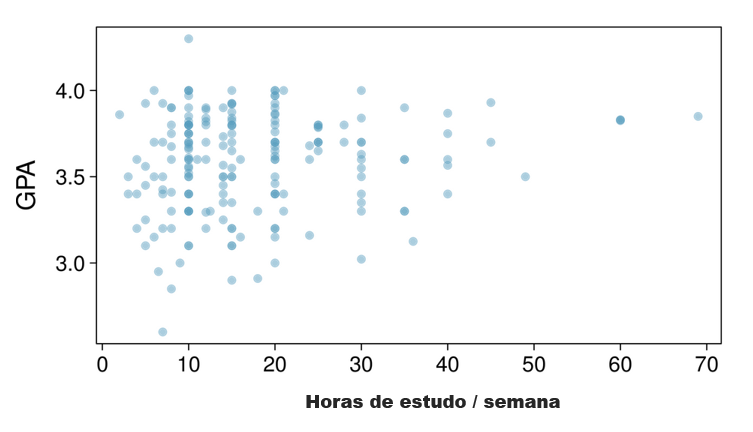
\includegraphics[scale=0.5]{1-2_data_basics/gpa_study_hours.png}
\end{center}

\end{frame}
%%%%%%%%%%%%%%%%%%%%%%%%%%%%%%%%%%%

\begin{frame}
\frametitle{Associação entre variáveis}

\dq{Você consegue identificar algo incomum?}

\soln{\pause{Há um aluno com GPA (nota) $> $ 4,0, isso é provavelmente um erro nos dados.}}

\end{frame}

%%%%%%%%%%%%%%%%%%%%%%%%%%%%%%%%%%%




\subsection{Variáveis dependentes e independentes}

%%%%%%%%%%%%%%%%%%%%%%%%%%%%%%%%%%%

\begin{frame}
\frametitle{Prática}

\twocol{0.5}{0.5}
{
\pq{Com base no gráfico de dispersão, qual das seguintes afirmações sobre comprimentos da cabeça e tamanho do crânio de gambás está correta?}
}
{
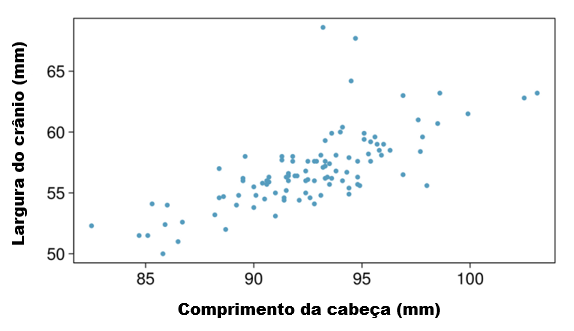
\includegraphics[width=0.7\textwidth]{1-2_data_basics/possum_head_skull.png}
}

\begin{enumerate}[(a)]
\justifying
\item Não existe relação entre o comprimento da cabeça e a largura do crânio, isto é, as variáveis são independentes.
\justifying
\solnMult{O comprimento da cabeça e a largura do crânio estão associadas positivamente.}
\justifying
\item A largura do crânio e o comprimento da cabeça estão associados negativamente.
\justifying
\item Uma cabeça mais longa faz com que o crânio fique mais largo.
\justifying
\item Um crânio mais largo faz com que a cabeça seja mais longa.
\end{enumerate}

\end{frame}

%%%%%%%%%%%%%%%%%%%%%%%%%%%%%%%%%%%

\begin{frame}
\frametitle{Associado vs. independente}

\begin{itemize}
\justifying
\item Quando duas variáveis mostram alguma conexão umas com as outras, elas podem ser chamadas de variáveis \hl{dependentes} e vice-versa.

\justifying
\item Se duas variáveis não estão associadas, ou seja, não há conexão evidente entre as duas, então elas são ditas \hl{independentes}.

\end{itemize}

\end{frame}

%%%%%%%%%%%%%%%%%%%%%%%%%%%%%%%%%%%%

%%%%%%%%%%%%%%%%%%%%%%%%%%%%%%%%%%%%

\section{1.3. Coleta dos dados}

%%%%%%%%%%%%%%%%%%%%%%%%%%%%%%%%%%%%

\subsection{Populações e amostras}

%%%%%%%%%%%%%%%%%%%%%%%%%%%%%%%%%%%%

\begin{frame}
\frametitle{Populações e amostras}


\begin{center}
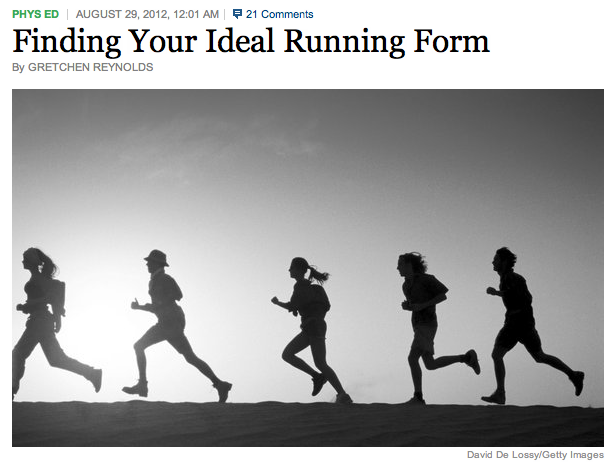
\includegraphics[width=0.5\textwidth]{1-3_data_collection_principles/figures/running.png}
\end{center}
\vspace{-0.5cm}
{\tiny \webURL{http://well.blogs.nytimes.com/2012/08/29/finding-your-ideal-running-form}}

\vspace{1cm}
\small{\textit{Tradução: Encontre sua corrida ideal.}}

\end{frame}
%%%%%%%%%%%%%%%%%%%%%%%%%%%%%%%%%%%%

\begin{frame}
\frametitle{Populações e amostras}
{
\justifying
\hl{Questão de pesquisa:} As pessoas podem se tornar corredores melhores e mais eficientes sozinhos, simplesmente correndo? \\
}
\vspace{0.5cm}
{
\justifying
\pause 
\justifying
\hl{População de interesse:} \soln{\pause Todas as pessoas.}
}
\pause 
\justifying
$\:$ \\
\vspace{0.5cm}
\justifying
\hl{Amostra:} Grupo de mulheres adultas que se juntaram recentemente a um grupo de corrida.\\
\vspace{0.5cm}
\pause
\justifying
\hl{População para a qual os resultados podem ser generalizados:} \soln{\pause Mulheres adultas, se os dados forem amostrados aleatoriamente.}

\end{frame}

%%%%%%%%%%%%%%%%%%%%%%%%%%%%%%%%%%%%

\subsection{Evidência anedótica}

%%%%%%%%%%%%%%%%%%%%%%%%%%%%%%%%%%%%

\begin{frame}
\frametitle{Evidência anedótica e pesquisa precoce sobre tabagismo}

\begin{itemize}
\justifying
\item A pesquisa antifumo começou nas décadas de 1930 e 1940, quando o consumo de cigarros se tornou cada vez mais popular. Enquanto alguns fumantes pareciam ser sensíveis à fumaça do cigarro, outros não eram afetados.
\vspace{0.5cm}
\justifying
\item A pesquisa anti-tabagismo foi confrontada com uma resistência baseada em \hl{evidências anedóticas} como "Meu tio fuma três maços por dia e está em perfeita saúde", evidência baseada em um tamanho de amostra limitado que pode não ser representativo da população.

\end{itemize}
\end{frame}

%%%%%%%%%%%%%%%%%%%%%%%%%%%%%%%%%%%%
\begin{frame}
\frametitle{Evidência anedótica e pesquisa precoce sobre tabagismo (cont.)}

\begin{itemize}
\justifying
\item Concluiu-se que "fumar é um comportamento humano complexo, por sua natureza difícil de estudar, confundido pela variabilidade humana".
\vspace{0.5cm}
\justifying
\item Com o tempo, os pesquisadores puderam examinar amostras maiores de casos (fumantes), e as tendências mostrando que fumar tem impactos negativos na saúde se tornaram muito mais claras.

\end{itemize}

\ct{Brandt, \textit{O século do cigarro} (2009), Livro Básico.}

\end{frame}

%%%%%%%%%%%%%%%%%%%%%%%%%%%%%%%%%%%%

\subsection{Amostragem de uma população}

\begin{frame}
\frametitle{Censo}

\begin{itemize}

\item Não seria melhor "amostrar" toda a população?

\begin{itemize}
\item Isso é chamado de \hl{censo}.
\end{itemize}

\pause

\item Há problemas em realizar um censo:

\begin{itemize}
\justifying
\item Pode ser difícil concluir um censo: sempre parece haver pessoas difíceis de localizar ou difíceis de avaliar. \textit{E essas pessoas difíceis de encontrar podem ter certas características que as distinguem do resto da população.}

\justifying
\item Populações raramente ficam paradas. Mesmo se você pudesse fazer um censo, a população muda constantemente, então nunca é possível obter uma medida perfeita.
\justifying
\item Fazer um censo pode ser mais complexo que a amostragem.
\end{itemize}

\end{itemize}

\end{frame}

%%%%%%%%%%%%%%%%%%%%%%%%%%%%%%%%%%%%%

\begin{frame}
\frametitle{Censo (cont.)}
\vfill

\begin{center}
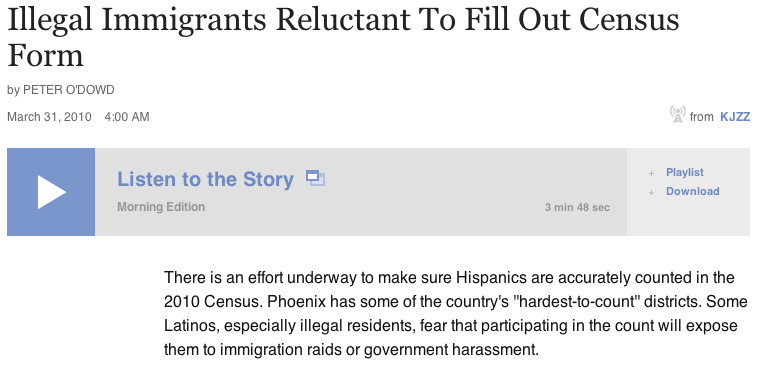
\includegraphics[width=0.50\textwidth]{1-3_data_collection_principles/figures/census_illegal_immig.png}
\end{center}

\ct{\webURL{http://www.npr.org/templates/story/story.php?storyId=125380052}}\\


\justifying
\small{
\hl{Tradução título:} Imigrantes ilegais relutam em preencher o formulário de recenseamento.\\
\justifying
\hl{Tradução texto:} Há uma pesquisa que busca  garantir que os hispânicos sejam contados com precisão no censo de 2010. Phoenix tem alguns dos distritos mais difíceis de serem pesquisados. Alguns latinos, especialmente moradores ilegais, temem que a participação na contagem os exponha a incursões na imigração ou a assédio do governo.}
\end{frame}

%%%%%%%%%%%%%%%%%%%%%%%%%%%%%%%%%%%%%

\begin{frame}
\frametitle{Análise exploratória e inferência}

\begin{itemize}

\item A amostragem é natural.

\pause

\justifying
\item Pense em provar algo que você está cozinhando - você prova (examina) uma pequena parte do que está cozinhando para ter uma ideia do prato como um todo.

\pause

\justifying
\item Quando você provar uma colherada de sopa e decidir que nesta colherada que você provou, falta sal, \hl{análise exploratória}.

\pause

\justifying
\item Se você generalizar e concluir que sua sopa inteira precisa de sal, isso é uma \hl{inferência}.

\pause
\end{itemize}

\end{frame}
%%%%%%%%%%%%%%%%%%%%%%%%%%%%%%%%%%%%%

\begin{frame}
\frametitle{Análise exploratória e inferência}

\begin{itemize}

\justifying
\item Para sua inferência ser válida, a colher que você provou (a amostra) precisa ser \hl{representativa} da panela inteira (a população).

\begin{itemize}
\justifying
\item Se a sua colherada vem apenas da superfície e o sal é coletado no fundo da panela, o que você provou provavelmente não é representativo da panela inteira.
\vspace{0.1cm}
\justifying
\item Se você primeiro misturar a sopa completamente antes de provar, sua colher será mais representativa da panela inteira.
\end{itemize}

\end{itemize}

\end{frame}

%%%%%%%%%%%%%%%%%%%%%%%%%%%%%%%%%%%%

\begin{frame}
\frametitle{Viés de amostragem}

\begin{itemize}
\justifying
\item \hl{Sem resposta:} Se apenas uma pequena fração das pessoas escolhidas aleatoriamente optar por responder a uma pesquisa, a amostra pode não ser mais representativa da população.
\vspace{0.1cm}
\pause
\justifying
\item \hl{Resposta voluntária:} Ocorre quando a amostra é constituída por pessoas que se voluntariam para responder porque têm opiniões fortes sobre o assunto. Essa amostra também não será representativa da população.

\end{itemize}

\end{frame}
%%%%%%%%%%%%%%%%%%%%%%%%%%%%%%%%%%%%

\begin{frame}
\frametitle{Viés de amostragem}

\begin{center}
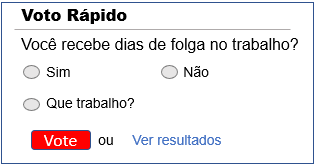
\includegraphics[width=0.5\textwidth]{1-3_data_collection_principles/vol_resp_bias_q.png}\pause
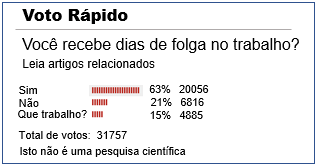
\includegraphics[width=0.5\textwidth]{1-3_data_collection_principles/vol_resp_bias_res.png} \\
{\tiny cnn.com, Jan 14, 2012}
\end{center}
\begin{itemize}
\pause
\justifying
\item \hl{Amostra de conveniência:} Indivíduos que são facilmente acessíveis têm maior probabilidade de serem incluídos na amostra.

\end{itemize}

\end{frame}

%%%%%%%%%%%%%%%%%%%%%%%%%%%%%%%%%%%%

\begin{frame}
\frametitle{Exemplo de viés de amostragem: Landon vs. FDR}
\justifying
Um exemplo histórico de uma amostra parcial que gera resultados enganosos: \\

$\:$ \\

\begin{columns}[c]

\column{0.35\textwidth}

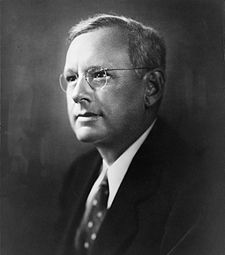
\includegraphics[width= \textwidth]{1-3_data_collection_principles/figures/landon_fdr/landon.png}

\column{0.3\textwidth}
\justifying
Em 1936, Landon buscou a indicação presidencial republicana contra a reeleição de FDR.

\column{0.35\textwidth}

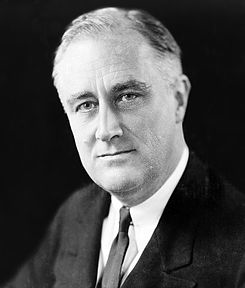
\includegraphics[width= \textwidth]{1-3_data_collection_principles/figures/landon_fdr/fdr.png}

\end{columns}

\end{frame}

%%%%%%%%%%%%%%%%%%%%%%%%%%%%%%%%%%%%%

\begin{frame}
\frametitle{A pesquisa de resumo literário}

\begin{columns}

\column{0.7\textwidth}

\begin{itemize}
\justifying
\item A revista Literary Digest entrevistou cerca de 10 milhões de americanos e obteve respostas de cerca de 2,4 milhões.
\justifying
\item A pesquisa mostrou que Landon provavelmente seria o grande vencedor da eleição e FDR receberia apenas 43 \% dos votos.

\item Resultado das eleições: FDR venceu com 62 \% dos votos.

\end{itemize}

\column{0.3\textwidth}

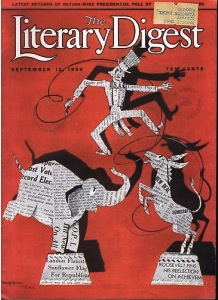
\includegraphics[width= \textwidth]{1-3_data_collection_principles/figures/literaryDigest.png}

\end{columns}

\begin{itemize}
\justifying
\item A revista ficou completamente desacreditada por causa da pesquisa e logo foi descontinuada.

\end{itemize}

\end{frame}

%%%%%%%%%%%%%%%%%%%%%%%%%%%%%%%%%%%%%

\begin{frame}
\frametitle{Sobre a pesquisa da revista Literary Digest - o que deu errado?}

\begin{itemize}

\item A revista havia pesquisado

\begin{itemize}

\item seus próprios leitores,

\item proprietários de automóveis registrados, e

\item usuários de telefone registrados.

\end{itemize}
\justifying
\item Esses grupos tinham rendimentos bem acima da média nacional da época (lembre-se, essa é a era da Grande Depressão) o que resultou em uma amostra de eleitores muito mais propensos a apoiar Landon, o que não representava o perfil eleitoral, ou seja, a amostra não era representativa da população americana na época.

\end{itemize}

\end{frame}

%%%%%%%%%%%%%%%%%%%%%%%%%%%%%%%%%%%%%

\begin{frame}
\frametitle{Amostras grandes são preferíveis, mas...}

\begin{itemize}
\justifying
\item A pesquisa eleitoral da Literary Digest  baseou-se em um tamanho de amostra de 2,4 milhões, o que é enorme, mas como a amostra era \bl {tendenciosa}, a amostra não produziu uma boa previsão.
\justifying
\item De volta à analogia da sopa: Se a sopa não estiver bem misturada, não importa quão grande seja a colher, ela ainda não terá o sabor certo. Se a sopa estiver bem misturada, uma colher pequena será suficiente para testar a sopa.

\end{itemize}

\end{frame}

%%%%%%%%%%%%%%%%%%%%%%%%%%%%%%%%%%%%%

\begin{frame}
\frametitle{Prática}
\justifying

\pq{Uma escola está considerando se permitirá que pais de alunos estacionem seus veículos na escola, depois de dois acidentes recentes. Como primeiro passo, eles enviam um e-mail aos pais e mães dos alunos, questionando se eles apoiariam essa mudança de política. De 6.000 e-mails, 1.200 são respondidos. Desses 1.200, 960 concordaram com a mudança de política e 240 discordaram. Qual das seguintes afirmações são verdadeiras?}
\end{frame}
%%%%%%%%%%%%%%%%%%%%%%%%%%%%%%%%%%%%%

\begin{frame}[shrink]
\frametitle{Prática}
\begin{enumerate}[I.]
\justifying
\item Alguns dos e-mails nunca foram recebidos pelos pais e pelas mães.
\justifying
\item Há forte concordância entre as famílias dos alunos, não deve-se permitir que estacionem o veículo  na escola.
\justifying
\item É possível que a maioria dos pais de alunos não esteja de acordo com essa mudança.
\justifying
\item É improvável que os resultados da pesquisa sejam parciais porque todos os pais receberam um e-mail.
\end{enumerate}


\justifying
\begin{multicols}{2}
\begin{enumerate}[(a)]
\item Somente I
\item I e II
\solnMult{I e III}
\item III e IV
\item Somente IV
\end{enumerate}
\end{multicols}


\end{frame}

%%%%%%%%%%%%%%%%%%%%%%%%%%%%%%%%%%%%%

\subsection{Variáveis explicativas e resposta}

%%%%%%%%%%%%%%%%%%%%%%%%%%%%%%%%%%%%%

\begin{frame}
\frametitle{Variáveis explicativas e de resposta}

\begin{itemize}
\justifying

\begin{center}
Variável explicativa $\xrightarrow{pode~afetar}$ variável resposta
\end{center}
\justifying
\item Rotular as variáveis como explicativas e respostas não garante que a relação entre as duas seja realmente causal, mesmo se houver uma associação identificada entre as duas variáveis. 

\end{itemize}

\end{frame}

%%%%%%%%%%%%%%%%%%%%%%%%%%%%%%%%%%%%%

\subsection{Estudos observacionais e experimentos aleatorizados}

%%%%%%%%%%%%%%%%%%%%%%%%%%%%%%%%%%%%%

\begin{frame}
\frametitle{Estudos observacionais e experimentos}

\begin{itemize}
\justifying
\item \hl{Estudos observacionais:} Os pesquisadores coletam dados de uma forma que não interfere diretamente na forma como os dados surgem, ou seja, eles apenas "observam", a interpretação dos resultados indicam associação entre as variáveis explicativas e respostas. Para avaliar a relação de causa e efeito é necessário estudos mais complexos, por meio de inferência causal. Essas técnicas não serão abordadas nesse curso.

\pause
\justifying
\item \hl{Experimentos:} Pesquisadores atribuem aleatoriamente sujeitos a vários tratamentos, a fim de estabelecer conexões causais entre as variáveis explicativas e de resposta.

\pause
\justifying
\item Lembre-se "correlação não implica causalidade".
\end{itemize}
\end{frame}
%%%%%%%%%%%%%%%%%%%%%%%%%%%%%%%%%%%%%

\begin{frame}
\frametitle{Estudos observacionais e experimentos}

\begin{center}
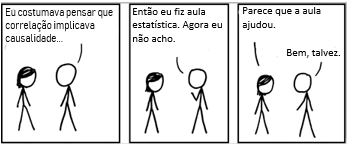
\includegraphics[width=0.7\textwidth]{1-3_data_collection_principles/xkcd_correlation.png} \\
{\tiny \webURL{http://xkcd.com/552/}}
\end{center}

\end{frame}

%%%%%%%%%%%%%%%%%%%%%%%%%%%%%%%%%%%%%


%%%%%%%%%%%%%%%%%%%%%%%%%%%%%%%%%%%%%

\section{1.4.Estudos observacionais e métodos de amostragem}

%%%%%%%%%%%%%%%%%%%%%%%%%%%%%%%%%%%%

\subsection{Confundindo}

%%%%%%%%%%%%%%%%%%%%%%%%%%%%%%%%%%%%

\begin{frame}
\frametitle{}

\begin{center}
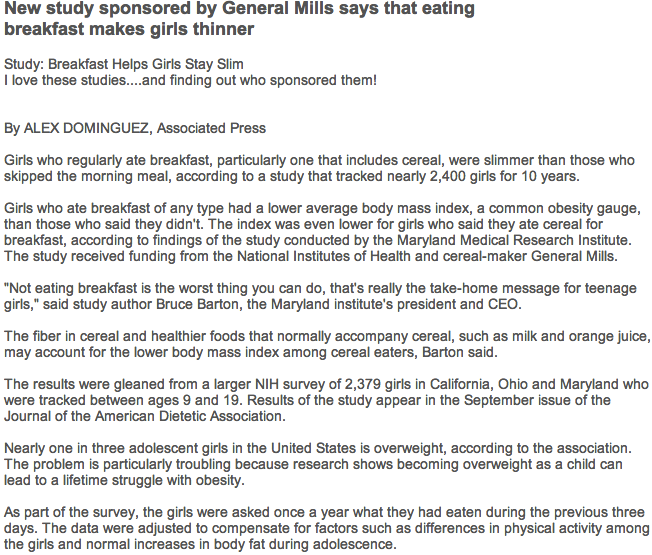
\includegraphics[width=0.80\textwidth]{1-4_obs_studies_sampling/figures/breakfast/breakfast1.png}
\end{center}

{\tiny \webURL{http://www.peertrainer.com/LoungeCommunityThread.aspx?ForumID=1\&ThreadID=3118}}

\end{frame}
%%%%%%%%%%%%%%%%%%%%%%%%%%%%%%%%%%%%

\begin{frame}
\frametitle{Tradução Texto}
\justifying
\tiny{
Novo estudo patrocinado pela General Mills diz que tomar o café da manhã deixa as meninas mais magras.\\
\vspace{0.2 cm}
Estudo: Café da manhã ajuda as meninas a permanecerem magras\\
\vspace{0.2 cm}
Eu amo esses estudos ... e descobrir quem os patrocinou!\\
\vspace{0.2 cm}
Por ALEX DOMINGUEZ, Jornalista associado.\\
\vspace{0.5 cm}
Garotas que tomam café da manhã regularmente, especialmente uma que inclui cereal, são mais magras do que as que pularam a refeição da manhã, de acordo com um estudo que acompanhou quase 2.400 garotas por 10 anos.\\

Meninas que tomavam o café da manhã de qualquer tipo tinham um índice de massa corporal médio menor, um índice de obesidade comum, daquelas que diziam que não o faziam. O índice foi ainda menor para as meninas que disseram que comeram cereais no café da manhã, de acordo com as conclusões do estudo realizado pelo Instituto de Pesquisa Médica de Maryland. O estudo recebeu financiamento do Instituto Nacional de Saúde e da fabricante de cereais General Mills.\\

"Não comer o café da manhã é a pior coisa que você pode fazer, é realmente a mensagem para as adolescentes", disse o autor do estudo, Bruce Barton, presidente e CEO do Instituto Maryland.\\

A fibra nos cereais e alimentos mais saudáveis que normalmente acompanham o cereal, como leite e suco de laranja, podem ser responsáveis pelo menor índice de massa corporal entre os consumidores de cereais, disse Barton.\\

Os resultados foram obtidos a partir de uma pesquisa maior do NIH com 2.379 meninas na Califórnia, Ohio e Maryland, que foram rastreadas entre as idades de 9 e 19 anos. Os resultados dos estudos aparecem na edição de setembro do Jornal da Associação Dietética Americana.\\

Quase uma em cada três adolescentes nos Estados Unidos têm sobrepeso, segundo a associação. O problema é particularmente preocupante porque a pesquisa mostra que o excesso de peso de uma criança pode levar a uma luta pela obesidade.\\

Como parte da pesquisa, as garotas foram perguntadas uma vez por ano o que haviam comido durante os três dias anteriores.\\

Os dados foram ajustados para compensar fatores como diferenças na atividade física entre as garotas e aumentos normais na gordura corporal durante a adolescência.
}

\end{frame}
%%%%%%%%%%%%%%%%%%%%%%%%%%%%%%%%%%%%

\begin{frame}
\frametitle{}
\justifying
\dq{Que tipo de estudo é este, estudo observacional ou um experimental?}\\
{\footnotesize \textit{``Garotas que tomam café da manhã regularmente, especialmente um que inclui cereal, são mais magras do que as que pularam a refeição, de acordo com o estudo que acompanhou quase 2.400 garotas por 10 anos.[...] Como parte da pesquisa, uma vez por ano as garotas respondiam um questionário sobre o que haviam comido durante os três dias anteriores."}}


\soln{\onslide<2->{Isto é um \hl{estudo observacional} já que os pesquisadores apenas observaram o comportamento das meninas (sujeitos) em oposição à imposição de tratamentos sobre elas.}}

\dq{Qual é a conclusão do estudo??}

\soln{\onslide<3->{Há uma \hl{associação} entre garotas serem magras e tomarem café da manhã.}}

\dq{Quem patrocinou o estudo?}

\soln{\onslide<4->{Todas}}

\end{frame}

%%%%%%%%%%%%%%%%%%%%%%%%%%%%%%%%%%%%

\begin{frame}[shrink]
\frametitle{3 explicações possíveis}

\pause

\begin{enumerate}

\item Comer o café da manhã faz com que as meninas fiquem mais magras.
\begin{center}
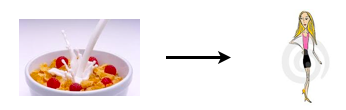
\includegraphics[width=0.5\textwidth]{1-4_obs_studies_sampling/figures/breakfast/breakfast2.png}
\end{center}

\pause

\item Ser magra faz com que as meninas tomem café da manhã.
\begin{center}

\includegraphics[width=0.5\textwidth]{1-4_obs_studies_sampling/figures/breakfast/breakfast3.png}
\end{center}

\pause
\justifying
\item Uma terceira variável é responsável por ambas. O que poderia ser? \\
Uma variável estranha que afeta tanto a variável explicativa quanto a variável de resposta e que faz parecer que existe uma relação entre as duas.
\begin{center}
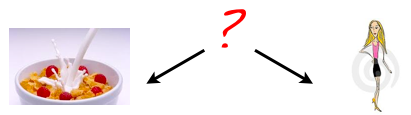
\includegraphics[width=0.5\textwidth]{1-4_obs_studies_sampling/figures/breakfast/breakfast4.png}
\end{center}

\end{enumerate}


{\tiny Images from: \webURL{http://www.appforhealth.com/wp-content/uploads/2011/08/ipn-cerealfrijo-300x135.jpg},  \webURL{http://www.dreamstime.com/stock-photography-too-thin-woman-anorexia-model-image2814892}.}



\end{frame}

%%%%%%%%%%%%%%%%%%%%%%%%%%%%%%%%%%%%

\begin{frame}
\frametitle{Estudos prospectivos vs. retrospectivos}

\begin{itemize}
\justifying
\item O estudo \hl{prospectivo} identifica indivíduos e coleta informações à medida que os eventos se desdobram.
\begin{itemize}
\justifying
\item Exemplo: Desde 1976 o Nurses Health Study (Estudo de Saúde para Enfermeiros nos EUA) tem recrutado enfermeiros e em seguida coletado dados por meio de questionários.
\end{itemize}
\justifying
\item \hl{Estudos retrospectivos} coletar dados após os eventos terem ocorrido.
\begin{itemize}
\justifying
\item Exemplo: Pesquisadores revisando eventos passados em registros médicos.
\end{itemize}

\end{itemize}

\end{frame}

%%%%%%%%%%%%%%%%%%%%%%%%%%%%%%%%%%%

\subsection{Métodos de amostragem}

%%%%%%%%%%%%%%%%%%%%%%%%%%%%%%%%%%%

\begin{frame}
\frametitle{Obtendo boas amostras}

\begin{itemize}
\justifying
\item Quase todos os métodos estatísticos são baseados na noção de aleatoriedade implícita.
\justifying
\item Se os dados observacionais não são coletados em uma estrutura aleatória, esses métodos estatísticos -- as estimativas e erros associados às estimativas -- não são confiáveis.
\justifying
\item As técnicas de amostragem aleatória mais comumente usadas são amostragem \hl{aleatória simples}, \hl{estratificado}, \hl{por conglomerados} e \hl{estratificada}.

\end{itemize}

\end{frame}

%%%%%%%%%%%%%%%%%%%%%%%%%%%%%%%%%%%%

\begin{frame}
\frametitle{Amostra aleatória simples}
\justifying
Seleciona aleatoriamente casos da população, onde não há conexão implícita entre os pontos selecionados.

\begin{center}
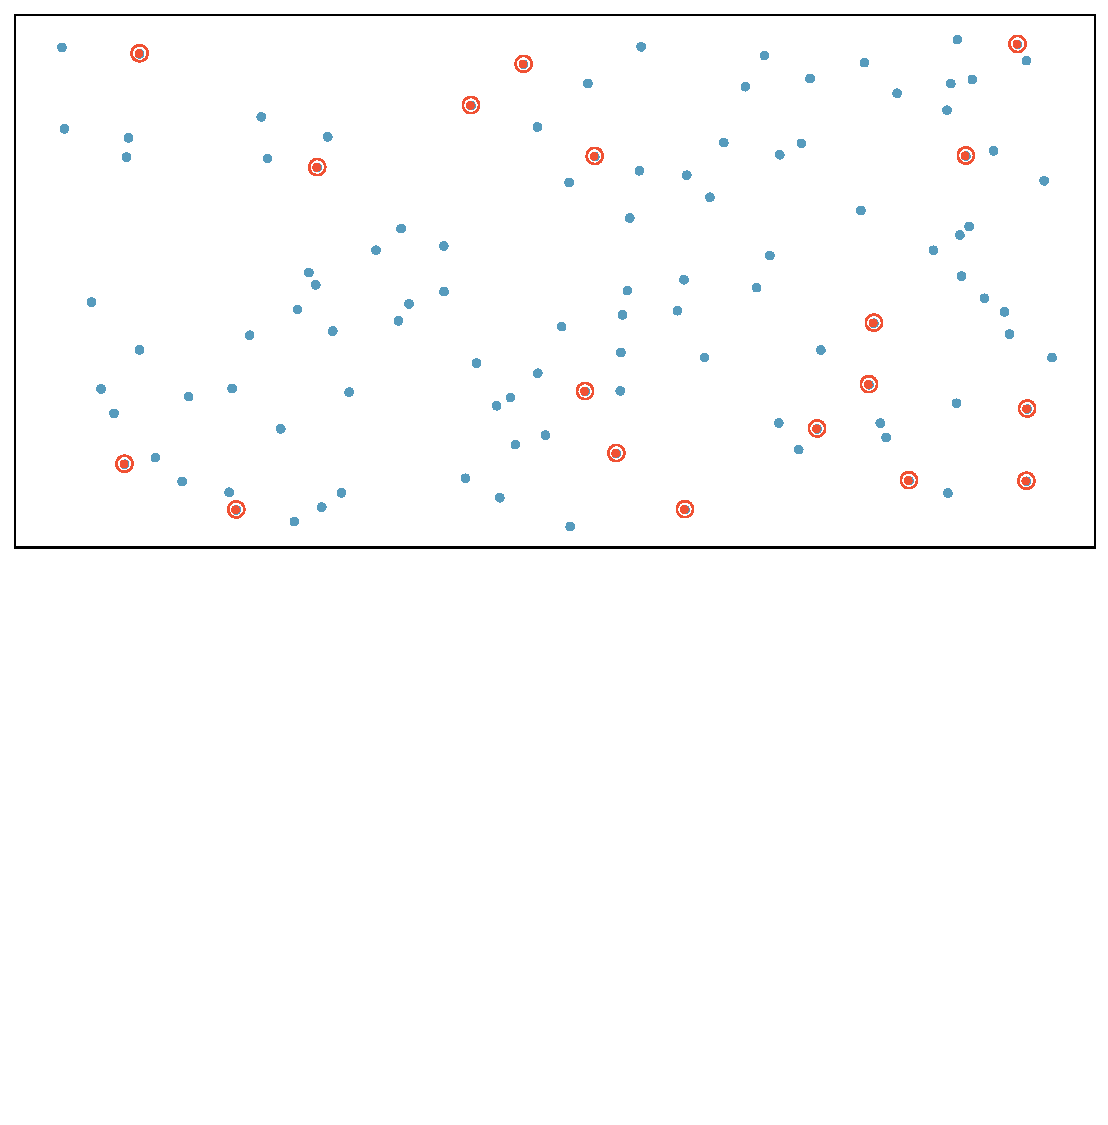
\includegraphics[width=0.9\textwidth]{1-4_obs_studies_sampling/simple.pdf}
\end{center}

\end{frame}

%%%%%%%%%%%%%%%%%%%%%%%%%%%%%%%%%%%%

\begin{frame}
\frametitle{Amostragem estratificada}
\justifying
\hl{Estratos} são constituídos por observações semelhantes. Seleciona-se uma amostra aleatória simples de \underline{cada} estrato.

\begin{center}
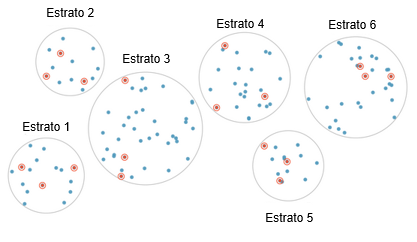
\includegraphics[width=0.9\textwidth]{1-4_obs_studies_sampling/stratified.png}
\end{center}

\end{frame}

%%%%%%%%%%%%%%%%%%%%%%%%%%%%%%%%%%%%

\begin{frame}
\frametitle{Amostragem por conglomerados}
\justifying
\hl{Grupos} geralmente não são feitos de observações homogêneas. Seleciona-se uma amostra aleatória simples dos conglomerados e, em seguida, \underline{todas} as observações nesse grupo. 

\begin{center}
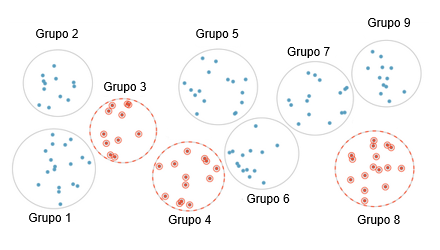
\includegraphics[width=0.9\textwidth]{1-4_obs_studies_sampling/cluster.png}
\end{center}

\end{frame}

%%%%%%%%%%%%%%%%%%%%%%%%%%%%%%%%%%%%

\begin{frame}
\frametitle{Amostragem em vários estágios}
\justifying
É comum quando se faz um plano amostral, utilizar os vários tipos de amostragem conjuntamente. Por exemplo, divide-se a população em conglomerados, tomamos uma amostra aleatória simples de grupos e, em seguida, obtemos uma amostra aleatória simples de observações dos grupos amostrados.

\begin{center}
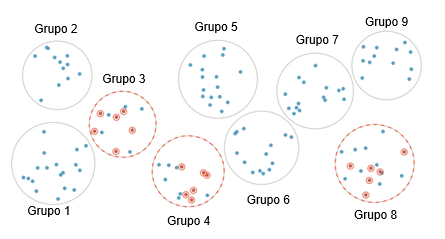
\includegraphics[width=0.9\textwidth]{1-4_obs_studies_sampling/multistage.png}
\end{center}

\end{frame}

%%%%%%%%%%%%%%%%%%%%%%%%%%%%%%%%%%%%

\begin{frame}
\frametitle{Prática}

\pq{
Um conselho municipal solicitou que uma pesquisa domiciliar fosse conduzida em uma área da cidade. A área é dividida em muitos bairros distintos, alguns incluindo grandes casas, alguns apenas com  apartamentos. Qual abordagem seria, provavelmente, \emph{menos} efetiva?}

\begin{enumerate}[(a)]
\item Amostragem aleatória simples
\solnMult{Amostragem por conglomerados}
\item Amostragem Estratificada
\item Amostragem sistemática.
\end{enumerate}

\end{frame}

%%%%%%%%%%%%%%%%%%%%%%%%%%%%%%%%%%%%


%%%%%%%%%%%%%%%%%%%%%%%%%%%%%%%%%%%%

\section{1.5.Experimentos}

%%%%%%%%%%%%%%%%%%%%%%%%%%%%%%%%%%%%
\begin{frame}
\frametitle{Princípios do delineamento experimental}

\begin{enumerate}
\justifying
\item \hl{Controle:} Compare o tratamento de interesse a um grupo controle.
\justifying
\item \hl{Aleatoriedade:} Atribui-se aleatoriamente os elementos ao grupo controle e grupo tratamento, além disso a amostra também deve ser aleatória.
\justifying
\item \hl{Blocos:} Se houver variáveis que são conhecidas ou suspeitas de afetar a variável de resposta, primeiro agrupe os sujeitos em \hl {blocos} com base nessas variáveis e, em seguida, faça a randomização aos grupo tratamento e controle dentro de cada bloco.

\end{enumerate}

\end{frame}

%%%%%%%%%%%%%%%%%%%%%%%%%%%%%%%%%%%%

\begin{frame}
\frametitle{Mais sobre os blocos}


\twocol{0.25}{0.75}
{
\begin{center}
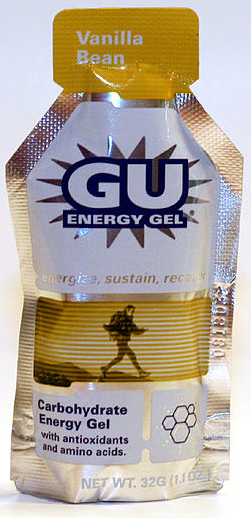
\includegraphics[width=\textwidth]{1-5_experiments/gu.png}
\end{center}
}
{
\begin{itemize}
\justifying
\item Gostaríamos de projetar um experimento para investigar se os géis de energia fazem você correr mais rápido:

\pause

\begin{itemize}
\item Tratamento: usar energy gel
\item Controle: não usar energy gel
\end{itemize}

\pause
\justifying
\item Suspeita-se que os géis de energia podem afetar os atletas profissionais e amadores de forma diferente, portanto, bloqueamos o status profissional:

\pause
\end{itemize}}
\end{frame}
%%%%%%%%%%%%%%%%%%%%%%%%%%%%%%%%%%%%

\begin{frame}
\frametitle{Mais sobre os blocos}

\begin{itemize}
   \begin{itemize}
   \justifying
\item Divida a amostra entre profissional e amador.
\justifying
\item Atribua aleatoriamente atletas profissionais a grupos de tratamento e controle.
\justifying
\item Atribua aleatoriamente atletas amadores para grupos de tratamento e controle.
\justifying
\item O status profissional/amador é igualmente representado nos grupos de tratamento e controle resultantes.
\end{itemize}
\end{itemize}


\pause

\dq{Por que isso é importante? Você pode pensar em outras variáveis para o bloco?}

\end{frame}

%%%%%%%%%%%%%%%%%%%%%%%%%%%%%%%%%%%%

\begin{frame}
\frametitle{Prática}
\justifying
\pq{Um estudo é projetado para testar o efeito do nível de luz e nível de ruído no desempenho de alunos em um exame. O pesquisador também acredita que os níveis de luz e ruído podem ter efeitos diferentes em homens e mulheres, portanto, quer garantir que ambos os gêneros estejam igualmente representados em cada grupo. Qual dos itens abaixo está correto?}
\small{
\begin{enumerate}[(a)]
\justifying
\item Existem 3 variáveis explicativas (luz, ruído, gênero) e 1 variável resposta (desempenho do exame).
\justifying
\solnMult{Existem 2 variáveis explicativas (luz e ruído), 1 variável de bloco (gênero) e 1 variável resposta (desempenho do exame)}
\justifying
\item Existe 1 variável explicativa (sexo) e 3 variáveis resposta (luz, ruído, desempenho do exame)
\justifying
\item Existem 2 variáveis de bloco (luz e ruído), 1 variável explicativa (sexo) e 1 variável de resposta (desempenho do exame)
\end{enumerate}
}
\end{frame}

%%%%%%%%%%%%%%%%%%%%%%%%%%%%%%%%%%%%

\begin{frame}
\frametitle{Diferença entre variáveis de bloqueio e explicativas}

\begin{itemize}
\justifying
\item Fatores são condições que podemos ser impostas nas unidades experimentais.
\justifying
\item As variáveis de bloqueio são características que as unidades experimentais têm e as quais gostaríamos de controlar.
\justifying
\item O bloqueio é como se fosse uma estratificação estratificação, exceto quando usado em configurações experimentais ao atribuir aleatoriamente, ao contrário de amostragem.

\end{itemize}

\end{frame}

%%%%%%%%%%%%%%%%%%%%%%%%%%%%%%%%%%%%

\begin{frame}
\frametitle{Mais terminologia de delineamento experimental ...}

\begin{itemize}
\justifying
\item \hl{Placebo:} tratamento falso, frequentemente usado como grupo de controle para estudos médicos.
\justifying
\item \hl{Efeito placebo:} unidades experimentais mostram melhora simplesmente porque acreditam que estão recebendo um tratamento especial.
\justifying
\item \hl{Cego:} quando as unidades experimentais não sabem se estão no grupo controle ou tratamento.
\justifying
\item \hl{Duplo-Cego:} quando tanto as unidades experimentais quanto os pesquisadores que interagem com os pacientes não sabem quem está no grupo controle e quem está no grupo tratamento.

\end{itemize}

\end{frame}

%%%%%%%%%%%%%%%%%%%%%%%%%%%%%%%%%%%%

\begin{frame}
\frametitle{Prática}
\justifying
\pq{Qual é a principal diferença entre estudos observacionais e experimentais?}

\begin{enumerate}[(a)]
\justifying
\item As experiências são realizadas em laboratório, enquanto os estudos observacionais não precisam de laboratório.
\justifying
\item Em um estudo observacional, observamos apenas o que aconteceu no passado.
\justifying
\solnMult{Estudos randomizados atribuem aleatoriamente os elementos ao grupo controle e ao grupo tratamento, enquanto os estudos observacionais não.}
\justifying
\item Estudos observacionais são completamente inúteis, uma vez que nenhuma inferência causal pode ser feita com base em seus achados.
\end{enumerate}

\end{frame}

%%%%%%%%%%%%%%%%%%%%%%%%%%%%%%%%%%%%


%%%%%%%%%%%%%%%%%%%%%%%%%%%%%%%%%%%%

\section{1.6. Estatística Descritiva, resumindo a informação contida}

%%%%%% d%%dade %os%%%%% no banco%%%%%%%%%%%%%%%%%%%%%%

\subsection{Gráficos de dispersão para dados pareados}

%%%%%%%%%%%%%%%%%%%%%%%%%%%%%%%%%%%%

\begin{frame}
\frametitle{Gráficos de dispersão}
\justifying
\hl{Gráficos de dispersão} são úteis para visualizar a relação entre duas variáveis numéricas.

\begin{columns}[c]

\column{0.6 \textwidth}
\justifying
\dq{A expectativa de vida e a fertilidade total parecem ser \hl {associadas} ou \hl {independentes}?}
\justifying
\soln{\onslide<2->{Eles parecem estar linearmente e negativamente associadas: à medida que a fertilidade aumenta, a expectativa de vida diminui.}}
\justifying
\dq{O associação foi a mesma ao longo dos anos, ou mudou?}
\justifying
\soln{\onslide<3->{A associação entre elas mudou ao longo dos anos.}}

\column{0.4 \textwidth}

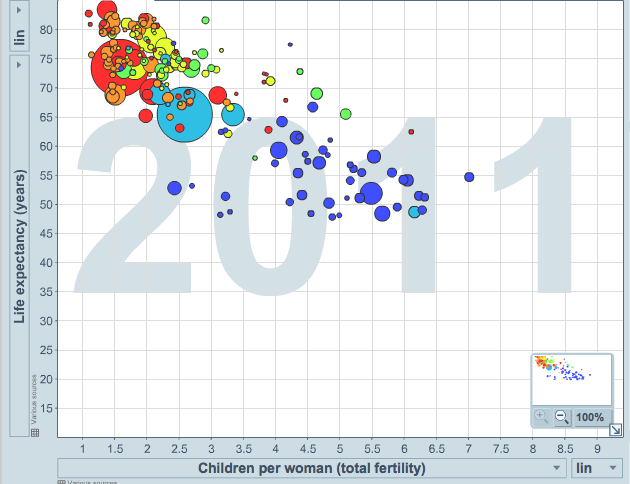
\includegraphics[width=\textwidth]{1-6_numerical_data/figures/life_exp_child.png}

\end{columns}

\ct{\webURL{http://www.gapminder.org/world}}

\end{frame}

%%%%%%%%%%%%%%%%%%%%%%%%%%%%%%%%%%%%

\subsection{Parcelas de pontos e a média}

%%%%%%%%%%%%%%%%%%%%%%%%%%%%%%%%%%%%

\begin{frame}
\frametitle{Gráfico}
\justifying
Útil para visualizar uma variável numérica. Cores mais escuras representam áreas onde há mais observações.

\begin{center}
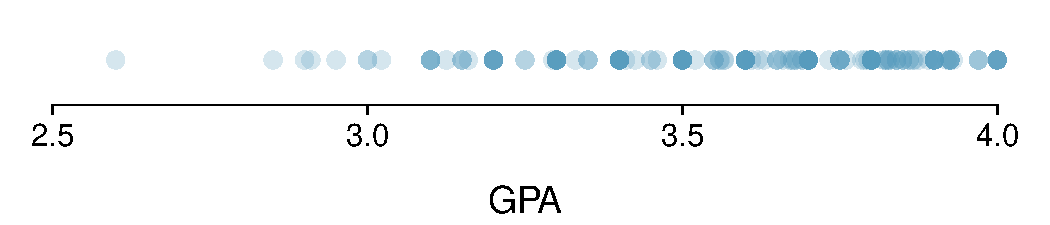
\includegraphics[width=\textwidth]{1-6_numerical_data/gpa_dot_plot.pdf}
\end{center}
\justifying
\dq{Como você descreveria a distribuição de GPAs nesse conjunto de dados? É possível indicar um ponto central ou a forma da distribuição desses dados?}

\end{frame}

%%%%%%%%%%%%%%%%%%%%%%%%%%%%%%%%%%%%


\begin{frame}
\frametitle{Gráfico}

\begin{center}
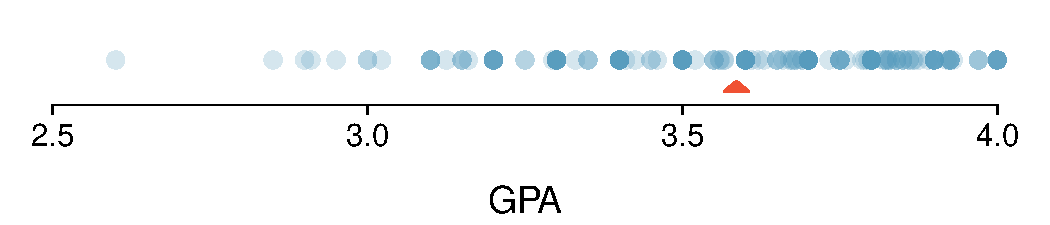
\includegraphics[width=\textwidth]{1-6_numerical_data/gpa_dot_plot_mean.pdf}
\end{center}

\begin{itemize}
\justifying
\item A \hl {média} (marcada com um triângulo no gráfico acima), é uma maneira de medir o centro de uma \hl {distribuição}.
\justifying
\item A média do GPA é de 3,59.

\end{itemize} 

\end{frame}

%%%%%%%%%%%%%%%%%%%%%%%%%%%%%%%%%%%%

\begin{frame}
\frametitle{Média}

\begin{itemize}
\justifying
\item A \hl {média da amostra}, denotada como \mathhl {\bar {x}}, pode ser calculada como

$$
\bar{x} = \frac{x_1 + x_2 + \cdots + x_n}{n},
$$

em que $x_1, x_2, \cdots, x_n$ representa as \hl{n} variáveis observadas.

\justifying
\item A \hl{média populacional} também é calculada da mesma maneira, mas é denotada como $\mathhl{\mu}$. Muitas vezes, não é possível calcular $\mu$, já que não temos informação sobre toda a população (censo).
\justifying
\item A média calculada com os dados da amostra é uma \hl{estatística} e serve como uma \hl{estimativa pontual} da média da população. Sua estimativa pode não ser perfeita, mas se a amostra for representativa da população, \hl{espera-se} que o resultado esteja próximo do verdadeiro valor populacional ($\mu$). 

\end{itemize}

\end{frame}

%%%%%%%%%%%%%%%%%%%%%%%%%%%%%%%%%%%%

\begin{frame}
\frametitle{Gráfico de pontos 2 }
\justifying
Barras mais altas representam áreas onde há mais observações, fica mais fácil visualizar o centro e a forma da distribuição.

\begin{center}
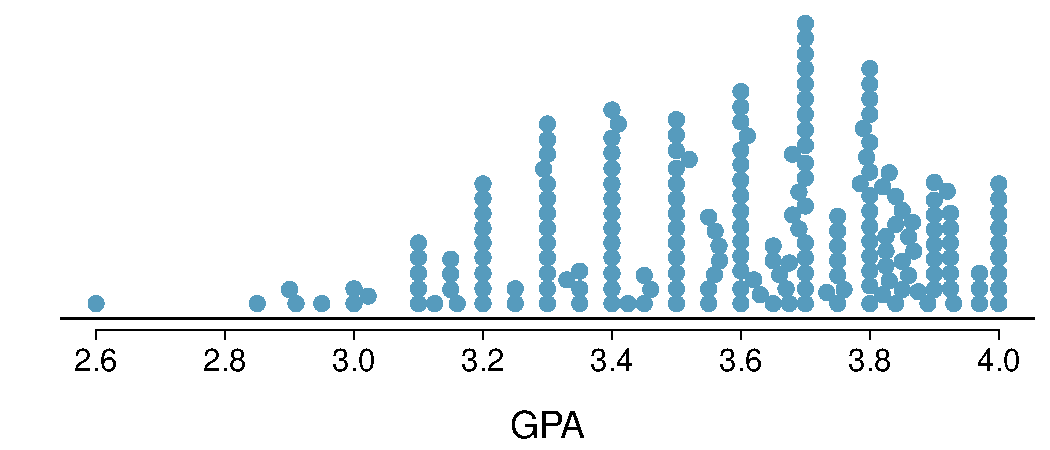
\includegraphics[width=\textwidth]{1-6_numerical_data/gpa_dot_plot_stacked.pdf}
\end{center}

\end{frame}

%%%%%%%%%%%%%%%%%%%%%%%%%%%%%%%%%%%%

\subsection{Histogramas}

%%%%%%%%%%%%%%%%%%%%%%%%%%%%%%%%%%%%

\begin{frame}[fragile]
\frametitle{Histogramas - horas extracurriculares}

\begin{itemize}
\justifying
\item Histogramas fornecem uma visão da \hl{densidade dos dados}. Barras mais altas representam onde os dados são relativamente mais comuns.
\justifying
\item Os histogramas são especialmente convenientes para descrever a \hl{forma} da distribuição dos dados.
\justifying
\item Importante destacar que dependendo da \hl{largura dos intervalos das caixas}, a história que o histograma está contando pode ser alterada drasticamente.

\end{itemize}

\begin{center}
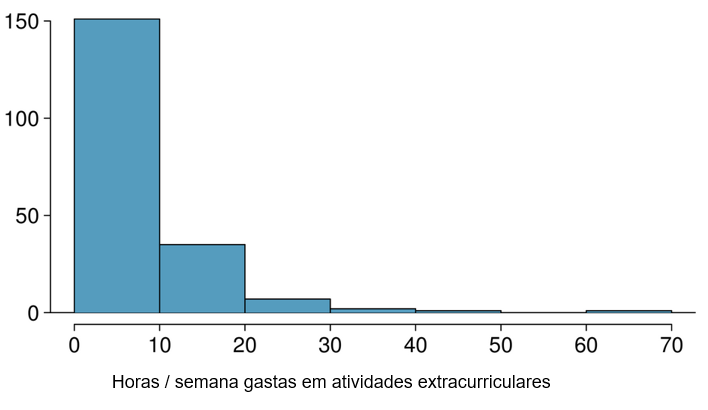
\includegraphics[width=0.60\textwidth]{1-6_numerical_data/extracurr_hrs_hist.png}
\end{center}

\end{frame}

%%%%%%%%%%%%%%%%%%%%%%%%%%%%%%%%%%%%

\begin{frame}
\frametitle{Largura dos intervalos das caixas}
\justifying
\dq{Qual (is) destes histogramas são úteis? Quais revelam muito sobre os dados? Quais escondem muito?}

\begin{center}
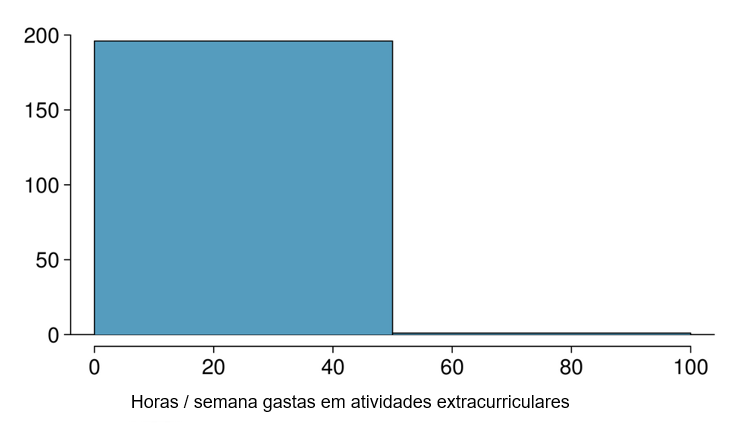
\includegraphics[width=0.45\textwidth]{1-6_numerical_data/extracurr_hrs_hist2.png}
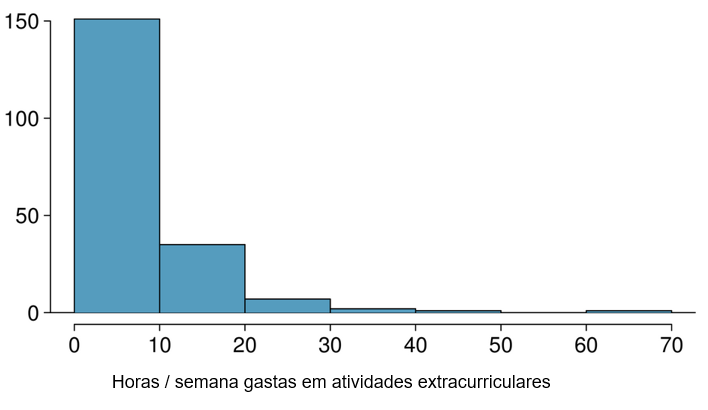
\includegraphics[width=0.45\textwidth]{1-6_numerical_data/extracurr_hrs_hist.png} \\
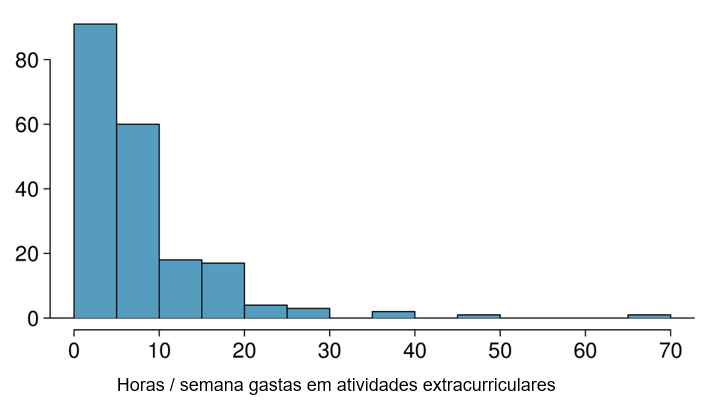
\includegraphics[width=0.45\textwidth]{1-6_numerical_data/extracurr_hrs_hist20.png}
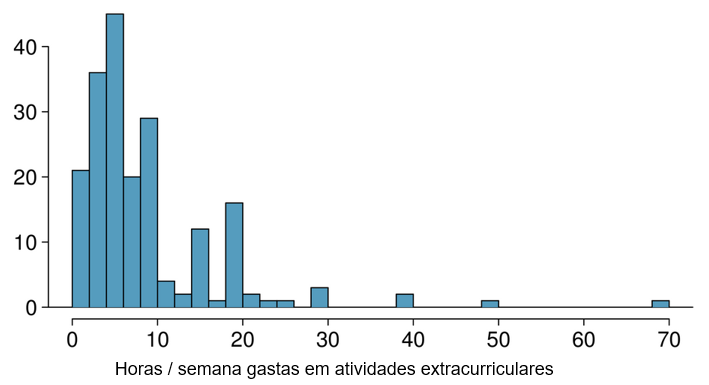
\includegraphics[width=0.45\textwidth]{1-6_numerical_data/extracurr_hrs_hist30.png}
\end{center}

\end{frame}

%%%%%%%%%%%%%%%%%%%%%%%%%%%%%%%%%%%%

\begin{frame}
\frametitle{Distribuição: moda}
\justifying
O histograma pode ter um único pico (\hl{unimodal}), vários picos proeminentes (\hl{bimodal/ multimodal}), ou sem picos aparentes (\hl{uniforme})?

\begin{center}
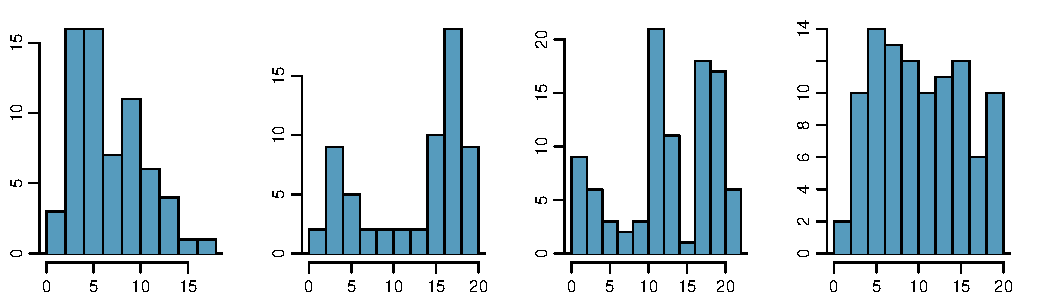
\includegraphics[width=0.75\textwidth]{1-6_numerical_data/singleBiMultiModalUnifPlots.pdf}
\end{center}
\justifying
\Note{Para determinar a moda,  imagine uma curva suave sobre o histograma - imagine que as barras sejam blocos de madeira e você jogue um espaguete mole sobre elas, a forma que o espaguete tomaria pode ser vista como uma curva suave.}

\end{frame}

%%%%%%%%%%%%%%%%%%%%%%%%%%%%%%%%%%%%

\begin{frame}
\frametitle{Distribuição: simetria}
\justifying
O histograma é \hl{assimétrico à direita}, \hl{assimétrico à esquerda}, ou \hl{simétrico}?

\begin{center}
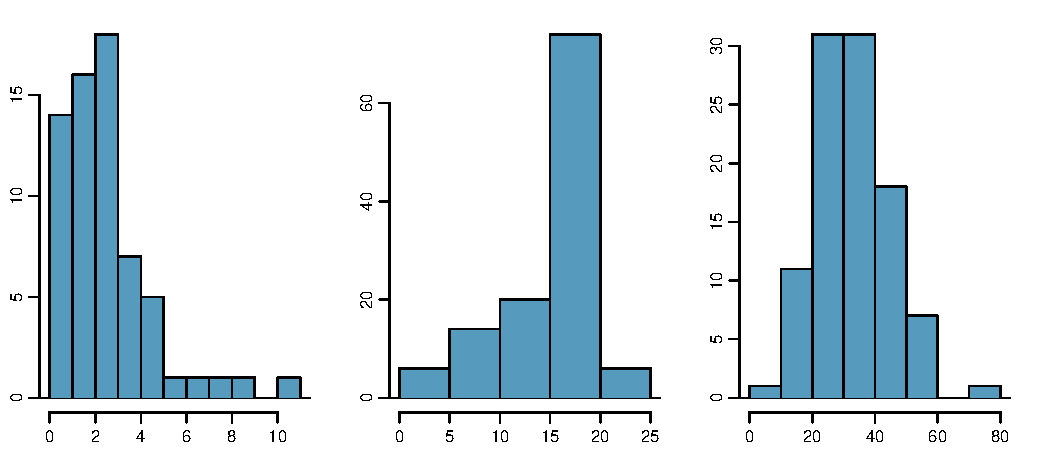
\includegraphics[width=0.8\textwidth]{1-6_numerical_data/skewedSymPlots.pdf}
\end{center}
\justifying
\Note{Observe para qual lado a calda da distribuição está.}

\end{frame}

%%%%%%%%%%%%%%%%%%%%%%%%%%%%%%%%%%%%

\begin{frame}
\frametitle{Forma de distribuição: observações incomuns}
\justifying
Há alguma observação incomum ou potencial \hl{outliers}?

\begin{center}
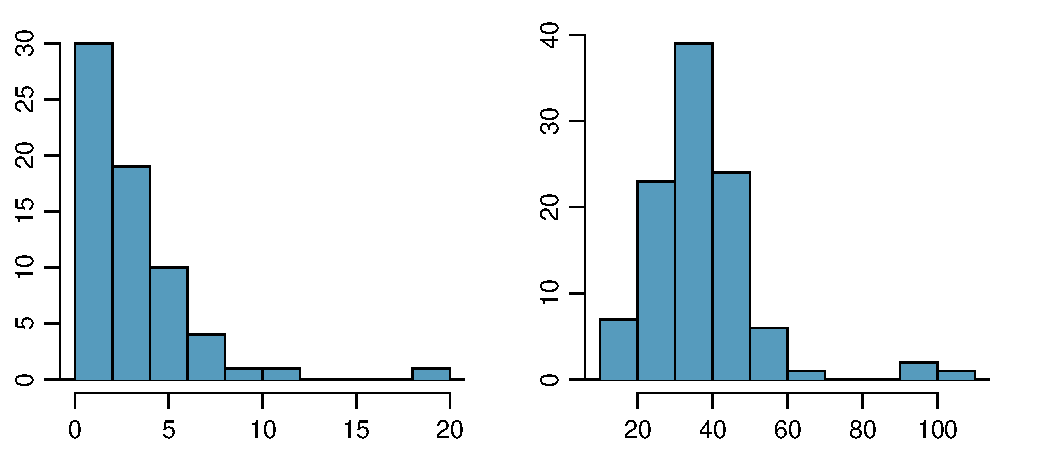
\includegraphics[width=0.8\textwidth]{1-6_numerical_data/outlierPlots.pdf}
\end{center}

\end{frame}

%%%%%%%%%%%%%%%%%%%%%%%%%%%%%%%%%%%%

\begin{frame}
\frametitle{Atividades extracurriculares}
\justifying
\dq{Como você descreveria a forma da distribuição das horas semanais em atividades extracurriculares de estudantes?}

\begin{center}
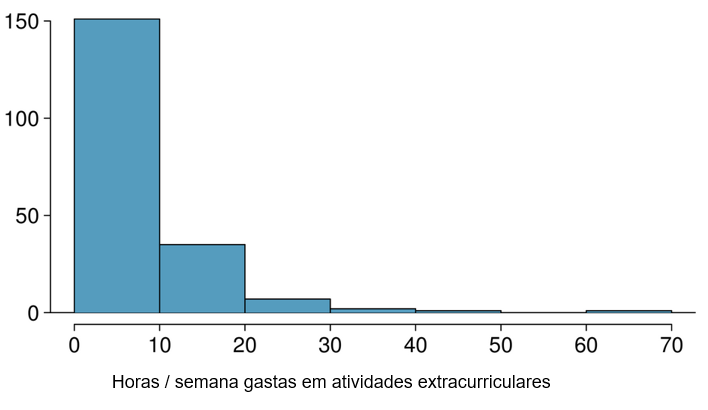
\includegraphics[width=0.75\textwidth]{1-6_numerical_data/extracurr_hrs_hist.png}
\end{center}
\justifying
\soln{\pause{Unimodal e assimétrica à direita. Outlier, às 60 horas/semana.}}

\end{frame}

%%%%%%%%%%%%%%%%%%%%%%%%%%%%%%%%%%%%

\begin{frame}
\frametitle{Formas comumente observadas de distribuições}

\begin{itemize}

\item modalidade \\
$\:$ \\
\pause

\begin{columns}[c]
\column{0.25\textwidth}
unimodal \\
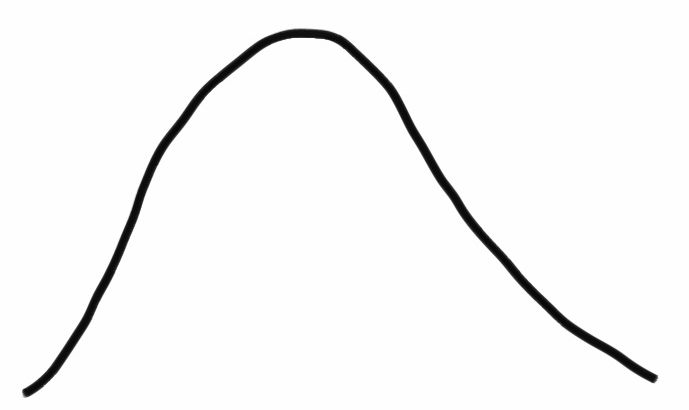
\includegraphics[width=\textwidth]{1-6_numerical_data/unimodal.png} 
\pause
\column{0.25\textwidth}
bimodal \\
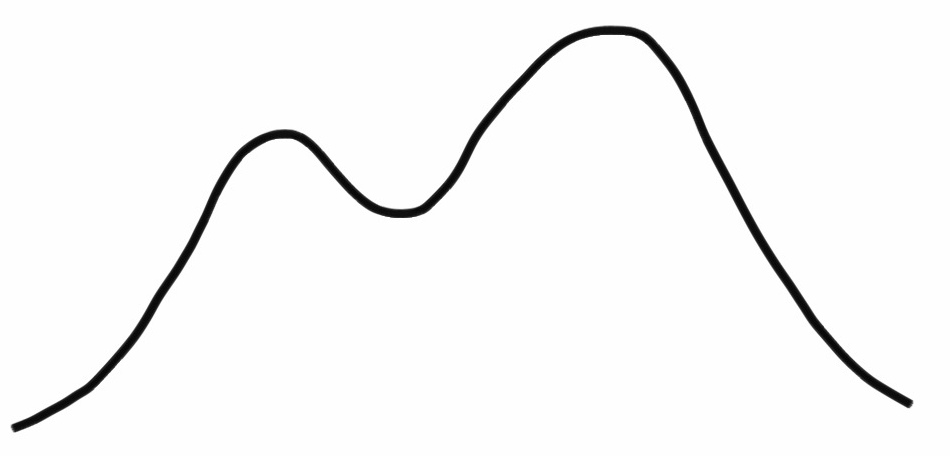
\includegraphics[width=\textwidth]{1-6_numerical_data/bimodal.png} 
\pause
\column{0.25\textwidth}
multimodal \\
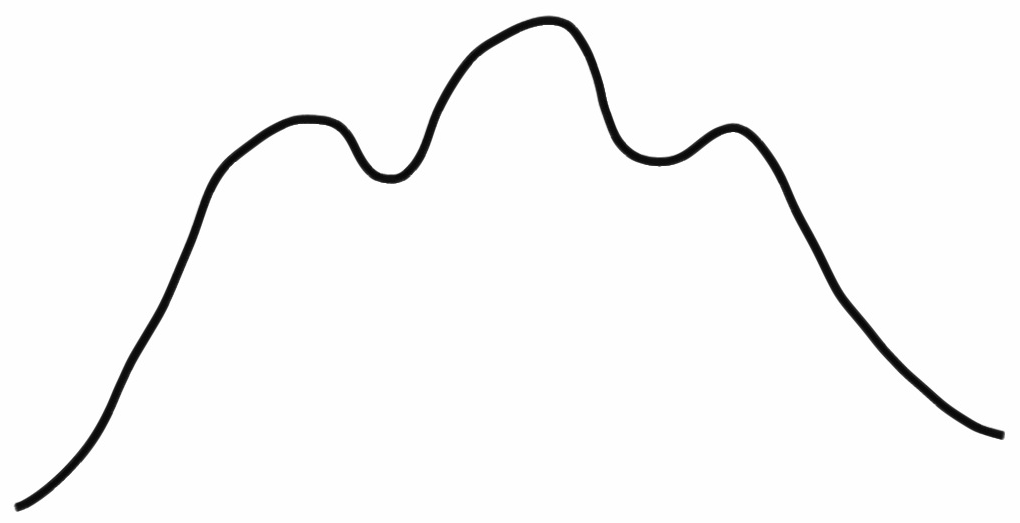
\includegraphics[width=\textwidth]{1-6_numerical_data/multimodal.png} 
\pause
\column{0.25\textwidth}
uniforme
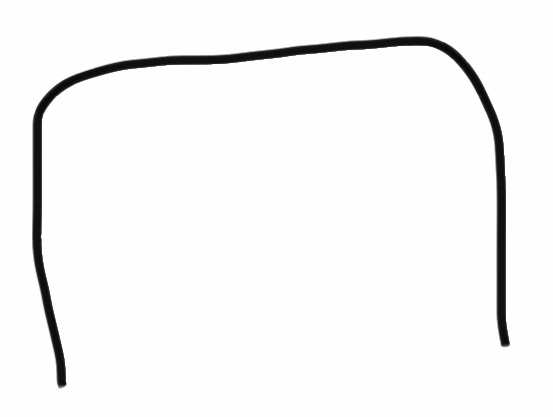
\includegraphics[width=\textwidth]{1-6_numerical_data/uniform.png} 
\end{columns}

\pause

$\:$ \\

\item assimétrica \\
$\:$ \\
\pause

\begin{columns}[c]
\column{0.25\textwidth}
à direita \\
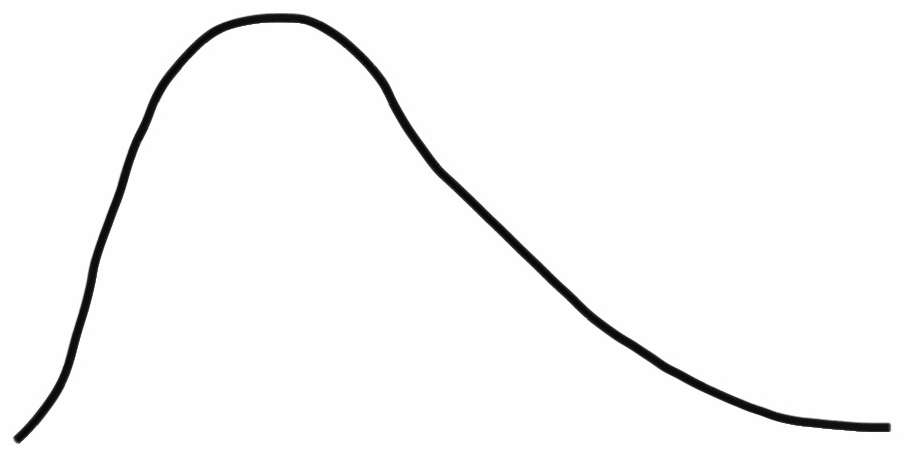
\includegraphics[width=\textwidth]{1-6_numerical_data/figures/shape_sketches/right_skew.png} 
\pause
\column{0.25\textwidth}
à esquerda \\
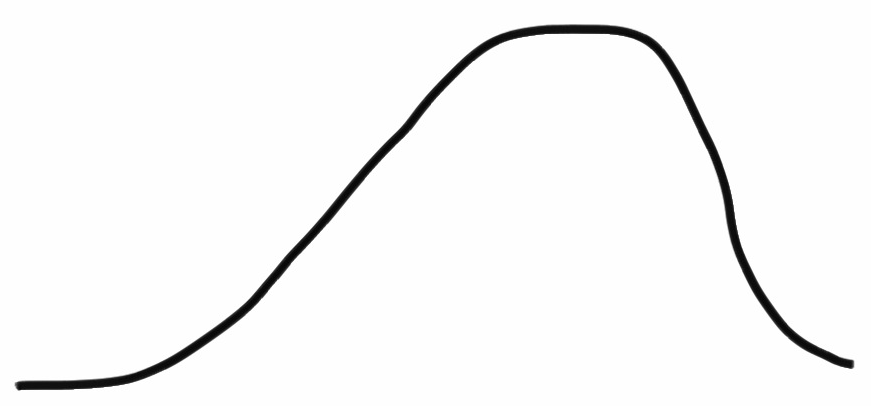
\includegraphics[width=\textwidth]{1-6_numerical_data/figures/shape_sketches/left_skew.png} 
\pause
\column{0.25\textwidth}
simétrico \\
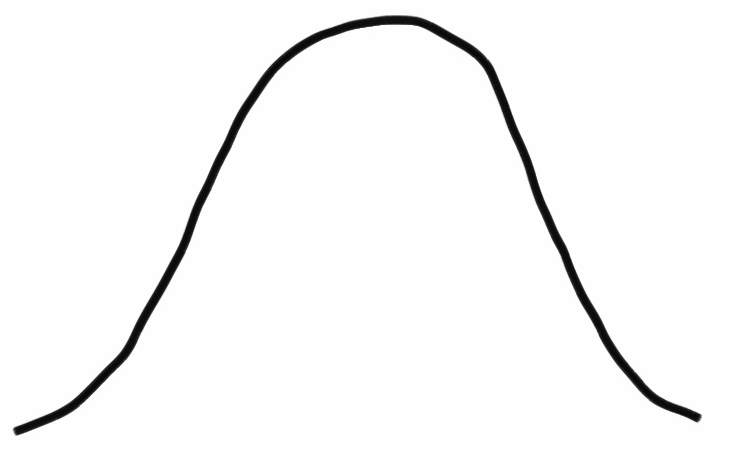
\includegraphics[width=\textwidth]{1-6_numerical_data/figures/shape_sketches/symmetric.png} 
\end{columns}

\end{itemize}

\end{frame}

%%%%%%%%%%%%%%%%%%%%%%%%%%%%%%%%%%%

\begin{frame}
\frametitle{Prática}

\pq{Quais dessas variáveis você espera que sejam uniformemente distribuídas?}

\begin{enumerate}[(a)]
\item pesos de habitantes de determinada cidade
\item salários de uma amostra aleatória de pessoas de Porto Alegre
\item Preços de casas
\solnMult{aniversários de colegas de turma (dia do mês)}
\end{enumerate}

\end{frame}

%%%%%%%%%%%%%%%%%%%%%%%%%%%%%%%%%%%

\begin{frame}
\frametitle{Atividade: formas de distribuições}

\app{Esboce as distribuições esperadas das seguintes variáveis:
\begin{itemize}
\item número de piercings
\item pontuações em um exame
\item Pontuações de QI
\end{itemize}
Invente uma maneira simples (1-2 sentenças) de ensinar alguém a determinar a distribuição esperada de qualquer variável.
}

\end{frame}

%%%%%%%%%%%%%%%%%%%%%%%%%%%%%%%%%%%

\begin{frame}
\frametitle{Você é típico? Qual seria o rosto médio de uma pessoa hoje?}

\begin{center}
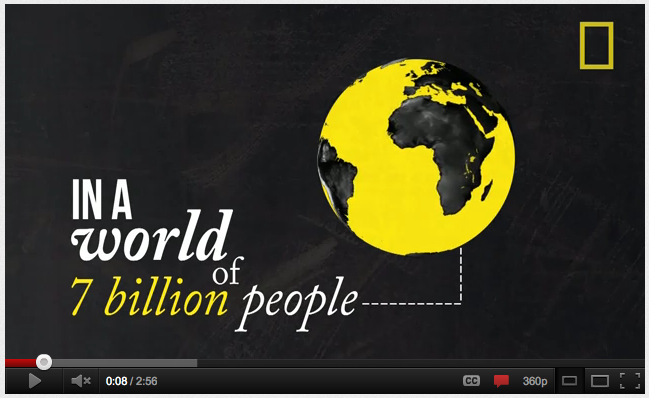
\includegraphics[width=0.75\textwidth]{1-6_numerical_data/figures/typical.png}
\end{center}

\begin{center}
\footnotesize{\webURL{http://www.youtube.com/watch?v=4B2xOvKFFz4}}
\end{center}


\end{frame}

%%%%%%%%%%%%%%%%%%%%%%%%%%%%%%%%%%%%

\subsection{Variância e desvio padrão}

%%%%%%%%%%%%%%%%%%%%%%%%%%%%%%%%%%%

\begin{frame}
\frametitle{Variância}
\justifying
\hl{Variância} é a soma dos desvios com relação à média ao quadrado.

\formula{
\[ s^2 = \frac{\sum_{i = 1}^n (x_i - \bar{x})^2}{n - 1} \]
}

\pause

\twocol{0.5}{0.5}
{
\begin{itemize}
\justifying
\item A média da amostra é $\bar{x} = 6,71$, e o tamanho da amostra é $n = 217$.
\justifying
\onslide<3->{\item A variação da quantidade de horas que estudantes dormem por noite pode ser calculada como:}
\end{itemize}
}
{
\onslide<2->{
\begin{center}
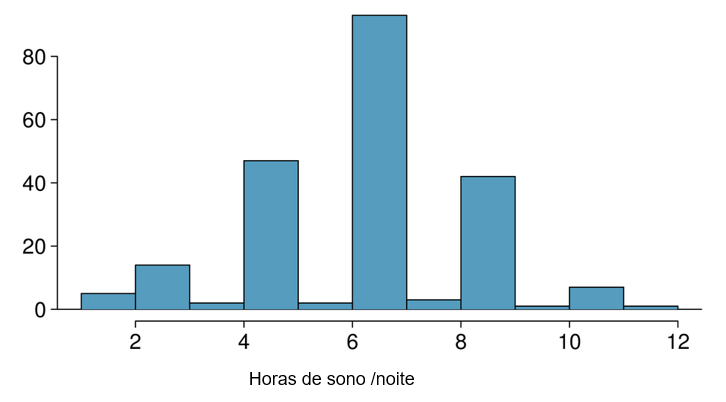
\includegraphics[width=\textwidth]{1-6_numerical_data/sleep_hist.png}
\end{center}
}
}
$\:$
\onslide<3->{
\[ s^2 = \frac{(5 - 6.71)^2 + (9 - 6.71)^2 + \cdots + (7 - 6.71)^2}{217 - 1} = 4.11~horas^2 \]
}



\end{frame}

%%%%%%%%%%%%%%%%%%%%%%%%%%%%%%%%%%%

\begin{frame}
\frametitle{Variância}
\justifying
\dq{Por que usamos o desvio ao quadrado no cálculo da variância?}

\soln{\pause
\begin{itemize}
\justifying
\item Para que as observações igualmente distantes da média sejam igualmente ponderadas, independentemente de essas distâncias serem positivas ou negativas.
\justifying
\item Para pesar desvios maiores mais fortemente.
\justifying
\item Porque as soma dos desvios em relação à média é zero


\end{itemize}
}

\end{frame}

%%%%%%%%%%%%%%%%%%%%%%%%%%%%%%%%%%

\begin{frame}
\frametitle{Desvio padrão}

\justifying
O \hl{desvio padrão} é a raiz quadrada da variância e possui a mesma unidade de medida dos dados observados.
$$
 s = \sqrt{s^2} 
$$
\pause
\twocol{0.5}{0.5}
{
\begin{itemize}
\justifying
\item O desvio padrão da quantidade de horas que estudantes dormem por noite é calculado como:
$$
 s = \sqrt{4.11} = 2.03~horas
$$
\justifying
\end{itemize}
}
{
\onslide<2->{
\begin{center}
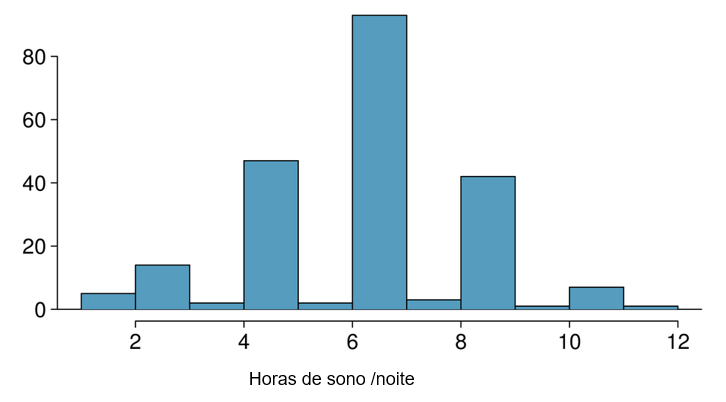
\includegraphics[width=\textwidth]{1-6_numerical_data/sleep_hist.png}
\end{center}
}
}

\end{frame}
%%%%%%%%%%%%%%%%%%%%%%%%%%%%%%%%%%

\begin{frame}
\frametitle{Desvio padrão}

\begin{itemize}
\justifying
$$
 s = \sqrt{4.11} = 2.03~horas
$$
\justifying
\item Observe que todas as observações estão dentro do intervalo de até 3 desvios padrões da média.
\end{itemize}
\begin{eqnarray*}
    (\overline{x}- 3s  &;& \overline{x}+ 3s)\\
     (6,71 -3\times2,03 &;& 6,71 +3\times2,03)
\end{eqnarray*}

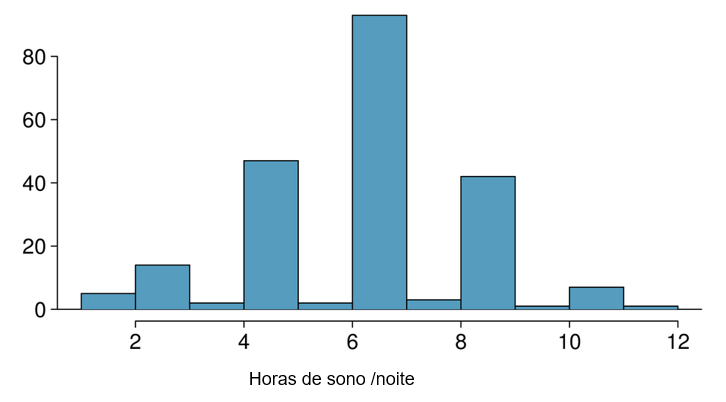
\includegraphics[width=6cm]{1-6_numerical_data/sleep_hist.png}

\end{frame}

%%%%%%%%%%%%%%%%%%%%%%%%%%%%%%%%%%%%

\subsection{Boxplot, quartis e a mediana}

%%%%%%%%%%%%%%%%%%%%%%%%%%%%%%%%%%%%

\begin{frame}
\frametitle{mediana}

\begin{itemize}
\justifying
\item A \hl{mediana} é o valor que divide  os dados ordenados pela metade.

\[ 0,1,\orange{2},3,4 \]
\justifying
\item Se houver um número par de observações, a mediana é a média dos dois valores do meio.

\[ 0,1,\underline{2,3},4,5 \rightarrow \frac{2 + 3}{2} = \orange{2.5} \]
\justifying
\item Como a mediana é o ponto médio dos dados, 50\% dos valores estão abaixo dela. Por isso, é também o \hl{percentil $50$}.

\end{itemize}

\end{frame}

%%%%%%%%%%%%%%%%%%%%%%%%%%%%%%%%%%%%

\begin{frame}[fragile]
\frametitle{Q1, Q3, and IQR}

\begin{itemize}
\justifying
\item O $25^{0}$ percentil também é chamado  primeiro quartil, \hl{Q1}.
\justifying
\item O $50^{0}$ percentil também é chamado de mediana.
\justifying
\item O $75^{0}$ percentil também é chamado terceiro quartil, \hl{Q3}.
\justifying
\item Entre Q1 e Q3 está 50\% dos dados. O intervalo desses dados é chamado de \hl{intervalo interquartílico} ou \hl{IQR}.

$$
IQR = Q3 - Q1 
$$

\end{itemize}

\end{frame}

%%%%%%%%%%%%%%%%%%%%%%%%%%%%%%%%%%%%

\begin{frame}
\frametitle{Boxplot}
\justifying
A caixa em um \hl{boxplot} representa 50\% dos dados e a linha que corta a caixa representa a \hl{mediana}.

\begin{center}
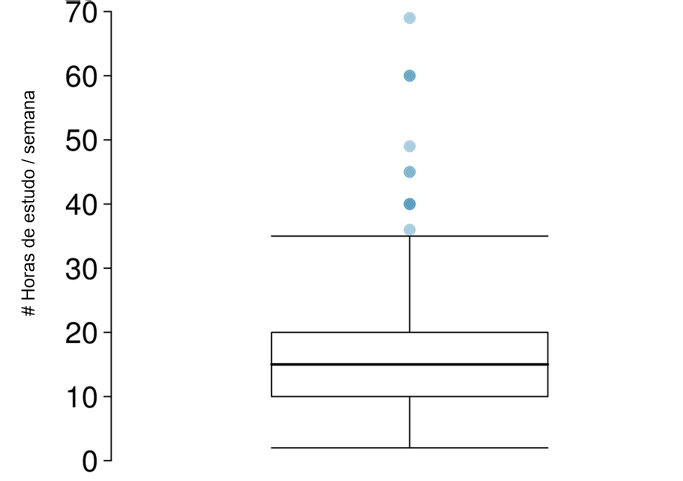
\includegraphics[width=0.7\textwidth]{1-6_numerical_data/study_hours_box.png}
\end{center}

\end{frame}

%%%%%%%%%%%%%%%%%%%%%%%%%%%%%%%%%%%%

\begin{frame}
\frametitle{Explicando um boxplot}

\begin{center}
\includegraphics[width=0.95\textwidth]{1-6_numerical_data/study_hours_box_layout.png}
\end{center}

\end{frame}

%%%%%%%%%%%%%%%%%%%%%%%%%%%%%%%%%%%%

\begin{frame}[fragile]
\frametitle{Bigodes e outliers}

\begin{itemize}
\justifying
\item \hl{Bigodes} de um gráfico de caixa podem se estender até $1.5 \times IQR$ longe dos quartis.\\
\formula{
\vspace{-0.5cm}
\begin{align*} 
\text{alcance~máximo~bigode~superior} &= Q3 + 1.5 \times IQR \\
\text{alcance~máximo~bigode~inferior~} &= Q1 - 1.5 \times IQR
\end{align*}
}
\pause
\vspace{-0.5cm}
{\small
\begin{align*}
\text{IQR}&: 20 - 10 = 10 \\
\text{alcance~máximo~bigode~superior}&= 20 + 1.5 \times 10 = 35 \\
\text{alcance~máximo~bigode~inferior}&= 10 - 1.5 \times 10 = -5
\end{align*}
}

\pause
\vspace{-0.25cm}
\justifying
\item Um potencial \hl{outlier} é definido como uma observação além do alcance máximo dos bigodes. É uma observação que parece extrema em relação ao resto dos dados.

\end{itemize}

\end{frame}

%%%%%%%%%%%%%%%%%%%%%%%%%%%%%%%%%%%%

\begin{frame}
\frametitle{Outliers (cont.)}
\justifying
\dq{Por que é importante procurar outliers?}

\soln{
\onslide<2->{
\begin{itemize}
\justifying
\item Identifica distorções na distribuição.
\justifying
\item Identifica erros ao construir o banco de dados e na coleta de dados.
\justifying
\item Fornece informações sobre características interessantes nos dados.
\end{itemize}
}
}

\end{frame}

%%%%%%%%%%%%%%%%%%%%%%%%%%%%%%%%%%%%

\subsection{Estatísticas robustas}

%%%%%%%%%%%%%%%%%%%%%%%%%%%%%%%%%%%%

\begin{frame}
\frametitle{Observações extremas}
\justifying
\dq{Como estatísticas como média, mediana, desvio padrão e IQR da renda familiar seriam afetadas se o maior valor fosse substituído por \$ 10 milhões? E se o menor valor fosse substituído por \$ 10 milhões?}

\begin{center}
\includegraphics[width=\textwidth]{1-6_numerical_data/house_income_dot_stacked.png}
\end{center}

\end{frame}

%%%%%%%%%%%%%%%%%%%%%%%%%%%%%%%%%%%%

\begin{frame}
\frametitle{Estatísticas robustas}

\begin{center}
\includegraphics[width=\textwidth]{1-6_numerical_data/house_income_dot_stacked.png}
\end{center}
\end{frame}
%%%%%%%%%%%%%%%%%%%%%%%%%%%%%%%%%%%%

\begin{frame}
\frametitle{Estatísticas robustas}

\begin{center}
\scalebox{0.9}{
\begin{tabular}{l c cc c cc}
  \hline

& \hspace{0mm} & \multicolumn{2}{c}{\bf robusta} & \hspace{2mm} & \multicolumn{2}{c}{\bf não robusta} \\
cenário && mediana & IQR && $\bar{x}$ & $s$ \\ 
  \hline
dados originais && 190K & 200K && 245K & 226K \\ 
substituir o maior valor por  && 190K & 200K && 309K & 853K \\
\$10 milhões & & & & \\
substituir o menor valor 
 && 200K & 200K && 316K & 854K \\
 por \$10 milhões & & & & \\
   \hline
\end{tabular}
}
\end{center}


\end{frame}

%%%%%%%%%%%%%%%%%%%%%%%%%%%%%%%%%%%%

\begin{frame}
\frametitle{Estatísticas robustas}
\justifying
A mediana e o IQR são mais robustas à assimetria e aos desvios do que a média e o desvio padrão. Assim sendo,

\begin{itemize}
\justifying
\item Para distribuições muito assimétricas, é mais útil usar mediana e IQR para descrever o centro e a variabilidade.
\justifying
\item Para distribuições simétricas, é mais útil usar a média e o desvio-padrão para descrever o centro e a variabilidade.
\end{itemize}

$\:$ \\

\pause
\justifying
\dq{Se você quiser estimar a renda familiar típica de um aluno, você estaria mais interessado na renda média ou mediana?}

\soln{\pause{Mediana}}

\end{frame}

%%%%%%%%%%%%%%%%%%%%%%%%%%%%%%%%%%%%

\begin{frame}
\frametitle{Média vs. mediana}

\begin{itemize}
\justifying
\item Se a distribuição é simétrica, o centro é geralmente definido como a média: média $\approx$ mediana

\begin{center}
\includegraphics[width=0.6\textwidth]{1-6_numerical_data/sym.png}
\end{center}

\end{itemize}

\end{frame}
%%%%%%%%%%%%%%%%%%%%%%%%%%%%%%%%%%%%

\begin{frame}
\frametitle{Média vs. mediana}

\begin{itemize}
\justifying
\item Se a distribuição é assimétrica ou tem outliers, o centro é geralmente definido como a mediana
\begin{itemize}
\item Assimétrico à direita: média $>$ mediana
\item Assimétrico à esquerda: média $<$ mediana \\
\end{itemize}

\end{itemize}

\begin{center}
\includegraphics[width=0.5\textwidth]{1-6_numerical_data/rs.png}
\includegraphics[width=0.5\textwidth]{1-6_numerical_data/ls.png}\\
\end{center}

\end{frame}

%%%%%%%%%%%%%%%%%%%%%%%%%%%%%%%%%%%%%

\begin{frame}
\frametitle{Prática}
\justifying
\pq{{\small O que é mais provável que seja verdade sobre a distribuição da porcentagem de tempo gasto com anotações em sala de aula em comparação com o Facebook, o Twitter etc.?}}

\vspace{-0.5cm}

\begin{columns}
\column{0.7\textwidth}
\begin{center}
\includegraphics[width=0.9\textwidth]{1-6_numerical_data/notes_perc_hist.png}
\end{center}
\column{0.3\textwidth}
$\:$ \\
$\:$ \\
\soln{\only<2>{\orange{mediana: 80\% \\ média: 76\%}}}
\end{columns}

{\small
\begin{multicols}{2}
\begin{enumerate}[(a)]
\item média $>$ mediana
\solnMult{média $<$ mediana}
\item média $\approx$ mediana
\item impossível dizer
\end{enumerate}
\end{multicols}
}

\end{frame}

%%%%%%%%%%%%%%%%%%%%%%%%%%%%%%%%%%%%%

\subsection{Transformando dados}

%%%%%%%%%%%%%%%%%%%%%%%%%%%%%%%%%%%%

\begin{frame}
\frametitle{Dados extremamente assimétricos}
\justifying
Quando os dados são extremamente assimétricos, transformá-los pode facilitar a modelagem. Uma transformação comum é a \hl{transformação log}.

$\:$ \\
\pause
\justifying
O histograma à esquerda mostra a distribuição do número de jogos de basquete assistidos pelos alunos. O histograma à direita mostra a distribuição do \hl{log} do número de jogos assistidos.

\begin{center}
\includegraphics[width=0.5\textwidth]{1-6_numerical_data/basket_games_hist.png}
\includegraphics[width=0.5\textwidth]{1-6_numerical_data/basket_games_hist_log.png}
\end{center}

\end{frame}

%%%%%%%%%%%%%%%%%%%%%%%%%%%%%%%%%%%%

\begin{frame}
\frametitle{Prós e contras de transformações}

\begin{itemize}
\justifying
\item Os dados assimétricos são mais fáceis de modelar quando são transformados, porque os outliers tendem a se tornar bem menos proeminentes após uma transformação apropriada. \\
$\:$ \\
\renewcommand{\arraystretch}{1.5}
\begin{tabular}{l r r r r }
\# de jogos		&  70 	& 50 		& 25 		 		& $\cdots$ \\
log(\# de jogos)	& 4.25	& 3.91 	& 3.22 	 	& $\cdots$
\end{tabular}

$\:$ \\
\justifying
\item No entanto, os resultados de uma análise podem ser difíceis de interpretar porque o \hl{log} de uma variável medida é geralmente sem sentido.

\end{itemize}

\pause
\justifying
\small{
\dq{Quais outras variáveis você esperaria que fossem extremamente assimétricas?}

\soln{\pause{Salário, preços de imóveis, etc.}}
}
\end{frame}

%%%%%%%%%%%%%%%%%%%%%%%%%%%%%%%%%%%%

\subsection{Mapeando dados}

%%%%%%%%%%%%%%%%%%%%%%%%%%%%%%%%%%%%

\begin{frame}
\frametitle{Mapas de intensidade}
\justifying
\dq{Quais padrões são aparentes na mudança de população entre 2000 e 2010?}

\begin{center}
\includegraphics[width=0.95\textwidth]{1-6_numerical_data/change_in_pop_intensity.png}
\end{center}

\ct{\webURL{http://projects.nytimes.com/census/2010/map}}

\end{frame}


%%%%%%%%%%%%%%%%%%%%%%%%%%%%%%%%%%%%



%%%%%%%%%%%%%%%%%%%%%%%%%%%%%%%%%%%%

\section{1.7.Dados categóricos}

%%%%%%%%%%%%%%%%%%%%%%%%%%%%%%%%%%%%

\subsection{Tabelas de Contingência e Gráficos de Barras}

%%%%%%%%%%%%%%%%%%%%%%%%%%%%%%%%%%%%

\begin{frame}
\frametitle{Tabelas de contingência}

\justifying
Uma tabela que resume a informação de duas variáveis categóricas é chamada de \hl {tabela de contingência}.

$\:$ \\
\pause
\justifying
A tabela de contingência abaixo mostra a distribuição dos gêneros dos alunos e se eles estão ou não procurando algum tipo de relacionamento durante a graduação.

\begin{center}
\begin{tabular}{l l cc rr}
					& 			& \multicolumn{2}{c}{{Procurando}} \\
  \cline{3-4}
					&			& Não	& Sim	& Total & \hspace{3mm}  \\ 
  \cline{2-5}
\multirow{2}{*}{{Gênero}}& Feminino 		& 86 	& 51 		& 137 \\ 
  					& Masculino 		& 52 	& 18	 	& 70\\ 
  \cline{2-5}
  					& Total		& 138& 69	&  207 \\
  \cline{2-5}
\end{tabular}
\end{center}

\end{frame}

%%%%%%%%%%%%%%%%%%%%%%%%%%%%%%%%%%%%

\begin{frame}
\frametitle{Gráficos de Barras}
\justifying
Um \hl {gráfico de barras} é uma maneira comum de exibir uma única variável categórica. Um gráfico de barras onde as proporções, em vez de frequências, são mostradas é chamado de \hl {barra de frequência relativa}.

\begin{center}
\includegraphics[width=0.45\textwidth]{1-7_categorical_data/gender_bar.png}
\includegraphics[width=0.45\textwidth]{1-7_categorical_data/gender_rel_bar.png}
\end{center}

\end{frame}
%%%%%%%%%%%%%%%%%%%%%%%%%%%%%%%%%%%%

\begin{frame}
\frametitle{Gráficos de Barras}
\dq{Qual a diferença entre gráfico de barras e histogramas?}
\justifying
\soln{\pause{{Gráficos de barra são usados para exibir distribuições de variáveis categóricas, enquanto histogramas são usados para variáveis numéricas. O eixo x em um histograma é uma linha numérica, portanto a ordem das barras não pode ser alterada, enquanto em um gráfico de barras as categorias podem ser listadas em qualquer ordem (embora algumas ordenações façam mais sentido que outras, especialmente para variáveis ordinais).
}}}

\end{frame}

%%%%%%%%%%%%%%%%%%%%%%%%%%%%%%%%%%

%%%%%%%%%%%%%%%%%%%%%%%%%%%%%%%%%%%%

\subsection{Proporções de linha e coluna}

%%%%%%%%%%%%%%%%%%%%%%%%%%%%%%%%%%%%

\begin{frame}
\frametitle{Escolhendo a proporção apropriada}
\justifying
\dq{Parece haver uma relação entre gênero e se o aluno está procurando algum relacionamento?}

\begin{center}
\begin{tabular}{l l cc r}
					& 			& \multicolumn{2}{c}{{Procurando }} \\
  \cline{3-4}
					&			& Não	& Sim	& Total \\ 
  \cline{2-5}
\multirow{2}{*}{{Gênero}}& Feminino 		& 86 	& 51 		& 137 \\ 
  					& Masculino 		& 52 	& 18	 	& 70\\ 
  \cline{2-5}
  					& Total		& 138& 69	&  207 \\
  \cline{2-5}
\end{tabular}
\end{center}

\pause
\justifying
Para responder a essa pergunta, examinamos as proporções nas linhas: 

\pause

\begin{itemize}
\justifying
\item \% Mulheres à procura de um relacionamento: $51 / 137 \approx 0.37$ \\

\pause
\justifying
\item \% Homens procurando por um relacionamento: $18 / 70 \approx 0.26$ \\

\end{itemize}

\end{frame}

%%%%%%%%%%%%%%%%%%%%%%%%%%%%%%%%%%%%

\subsection{Barras segmentadas e mosaicos}

%%%%%%%%%%%%%%%%%%%%%%%%%%%%%%%%%%%%

\begin{frame}
\frametitle{Barras segmentadas e mosaicos}
\justifying
\dq{Abaixo os gráficos respresentando a tabela do slide anterior. Quais são as diferenças entre as três visualizações mostradas abaixo?}

\begin{center}
\includegraphics[width=0.33\textwidth]{1-7_categorical_data/gender_seg_bar.png}
\includegraphics[width=0.33\textwidth]{1-7_categorical_data/gender_rel_seg_bar.png}
\includegraphics[width=0.33\textwidth]{1-7_categorical_data/gender_mosaic.png}
\end{center}

\end{frame}

%%%%%%%%%%%%%%%%%%%%%%%%%%%%%%%%%%%%

\subsection{Gráfico de setores}

%%%%%%%%%%%%%%%%%%%%%%%%%%%%%%%%%%%%

\begin{frame}
\frametitle{Gráfico de setores}
\justifying
\dq{Você pode dizer qual grupo engloba a menor porcentagem de espécies de mamíferos?}

\vspace{-0.5cm}

\begin{center}
\includegraphics[width=0.4\textwidth]{1-7_categorical_data/mammal_pie_chart.pdf}
\includegraphics[width=0.2\textwidth]{1-7_categorical_data/mammal_pie_chart_legend.pdf}
\end{center}
\justifying
\ct{Dados de \webURL{http://www.bucknell.edu/msw3}.}

\end{frame}


%%%%%%%%%%%%%%%%%%%%%%%%%%%%%%%%%%%%

\subsection{Comparando dados numéricos entre grupos}

%%%%%%%%%%%%%%%%%%%%%%%%%%%%%%%%%%%%

\begin{frame}
\frametitle{Gráfico de boxplot lado a lado}
\justifying
\dq{Parece haver uma relação entre o ano da turma e o número de clubes frequentados pelos alunos?}

\begin{center}
\includegraphics[width=\textwidth]{1-7_categorical_data/year_clubs.png}
\end{center}
%%%%MUDARRR
\end{frame}

%%%%%%%%%%%%%%%%%%%%%%%%%%%%%%%%%%%%



\section{1.8. Estudo de caso: discriminação de gênero}

%%%%%%%%%%%%%%%%%%%%%%%%%%%%%%%%%%%%

\subsection{Descrição e dados do estudo}

%%%%%%%%%%%%%%%%%%%%%%%%%%%%%%%%%%%%

\begin{frame}
\frametitle{Discriminação de gênero}

\begin{itemize}
\justifying
\item Em 1972, como parte de um estudo sobre discriminação de gênero, 48 supervisores bancários (homens) receberam o mesmo currículo de um candidato a gerente de uma filial, os supervisores deveriam sugerir se a pessoa deveria ser promovida. 
\justifying
\item Os currículos eram idênticos, exceto que, metade deles o candidato a promoção era do sexo masculino, enquanto a outra metade tinha currículos mostrando que a pessoa era do sexo feminino.
\justifying
\item Foi determinado aleatoriamente quais supervisores receberiam currículos "masculinos" e quais supervisores receberiam currículos "femininos".  
\end{itemize}
\end{frame}
%%%%%%%%%%%%%%%%%%%%%%%%%%%%%%%%%%%%

\begin{frame}
\frametitle{Discriminação de gênero}

\begin{itemize}
\justifying
\item Dos 48 currículos analisados, 35 foram promovidos. 
\justifying
\item O estudo tem como objetivo avaliar se as mulheres são discriminadas injustamente.  
\end{itemize}
\justifying
\dq{Isto é um estudo observacional ou experimental?} \soln{\onslide<2->{Experimento}}
\justifying
\ct{B.Rosen and T. Jerdee (1974), ``nfluência de estereótipos de papéis sexuais nas decisões de pessoal", J.Applied Psychology, 59:9-14.}

\end{frame}


%%%%%%%%%%%%%%%%%%%%%%%%%%%%%%%%%%%%

\begin{frame}
\frametitle{Dados}
\justifying
\dq{À primeira vista, parece haver uma relação entre promoção e gênero?}

\begin{center}
\begin{tabular}{ll  cc c} 
  		&				& \multicolumn{2}{c}{\textit{Promoção}} \\
\cline{3-4}
							&			& Promovido	& Não Promovido 	& Total	\\
\cline{2-5}
\multirow{2}{*}{\textit{Gênero	}}	&Masculino 		& 21	 	& 3		& 24 	\\
							&Feminino		& 14	 	& 10 	 	& 24 \\
\cline{2-5}
							&Total		& 35		& 13		& 48 \\
\end{tabular}
\end{center}

\pause

\textbf{\% de homens promovidos: $21 / 24 = 0.875$} \\
\textbf{\% de mulheres promovidas: $14 / 24 = 0.583$}

\end{frame}

%%%%%%%%%%%%%%%%%%%%%%%%%%%%%%%%%%%%

\begin{frame}
\frametitle{Prática}
\justifying
\pq{Vimos uma diferença de quase 30\% (29,2\% para ser exato) entre a proporção de currículos de homens e mulheres que seriam promovidos. Com base nessas informações, qual das alternativas abaixo é verdadeira?}
\vspace{-0.5cm}
\small{
\begin{enumerate}[(a)]
\justifying
\item Se fôssemos repetir a experiência, definitivamente veremos que mais mulheres são promovidas. Isso foi o acaso.
\justifying
\item A promoção depende do gênero, os homens têm maior chance de serem promovidos independentemente do currículo, portanto, há discriminação de gênero contra as mulheres nas decisões de promoção. \soln{\only<2>{\red{Talvez}}}
\justifying
\item A diferença na proporção de homens e mulheres a serem promovidos é devido ao acaso, isto não é evidência de discriminação de gênero contra mulheres em decisões de promoção. \soln{\only<2>{\red{Talvez}}}
\justifying
\item As mulheres são menos qualificadas do que os homens, é por isso que menos mulheres são promovidas.

\end{enumerate}
}
\end{frame}

%%%%%%%%%%%%%%%%%%%%%%%%%%%%%%%%%%%%

\subsection{Suposições}

%%%%%%%%%%%%%%%%%%%%%%%%%%%%%%%%%%%%%

\begin{frame}
\frametitle{Duas suposições concorrentes}

\begin{enumerate}
\justifying
\item `` Não há nada acontecendo." \\
\justifying
Promoção e gênero são \hl{independentes}, não há discriminação de gênero, a diferença observada nas proporções é devida, simplesmente,  ao acaso. $\rightarrow$ \hl{Hipótese nula}

\pause
\justifying
\item `` Há algo acontecendo." \\
\justifying
Promoção e gênero são \hl {dependentes}, há discriminação de gênero, a diferença observada nas proporções não se deve ao acaso. $\rightarrow$ \hl{Hipótese alternativa}

\end{enumerate}

\end{frame}

%%%%%%%%%%%%%%%%%%%%%%%%%%%%%%%%%%%%

\begin{frame}
\frametitle{Um julgamento pensado como um teste de hipóteses}

\twocol{0.5}{0.5}
{
\begin{itemize}
\justifying
\item O teste de hipóteses é muito parecido com um julgamento no tribunal.
\justifying
\item $H_0$: Réu é inocente \\
$H_A$: Réu é culpado
\justifying
\item Em seguida, apresentamos as evidências - coletamos dados.

\end{itemize}
}
{
\includegraphics[width=\textwidth]{1-8_gender_discrimination/trial.png}
}

\begin{itemize}
\justifying
\item Então, julgamos as evidências - "Esses dados poderiam ter ocorrido por acaso, se a hipótese nula fosse verdadeira?"
\begin{itemize}
\justifying
\item Se é muito improvável que tenhamos observado determinado conjunto de dados dado que a hipótese nula é verdadeira, as evidências levantam mais do que uma dúvida razoável em nossas mentes. \pause Será que minha suposição inicial, a hipótese nula, é verdade? 
\end{itemize}
\end{itemize}
\end{frame}
%%%%%%%%%%%%%%%%%%%%%%%%%%%%%%%%%%%%

\begin{frame}
\frametitle{Um julgamento pensado como um teste de hipóteses}
\begin{itemize}
\justifying
\item Em última análise, devemos tomar uma decisão. Quão improvável?

\end{itemize}
\justifying
\includegraphics[width=5cm]{1-8_gender_discrimination/trial.png}

\ct{Imagem de \webURL{http://www.nwherald.com/_internal/cimg!0/oo1il4sf8zzaqbboq25oevvbg99wpot}.}

\end{frame}

%%%%%%%%%%%%%%%%%%%%%%%%%%%%%%%%%%%%%

\begin{frame}
\frametitle{Um julgamento pensado como um teste de hipóteses (cont.)}

\begin{itemize}
\justifying
\item Se a evidência não for forte o suficiente para rejeitar a suposição de inocência, o júri retorna com um veredicto de "não culpado".
\begin{itemize}
\justifying
\item O júri não diz que o réu é inocente, apenas que não há provas suficientes para condenar.
\justifying
\item O réu pode, de fato, ser inocente, mas o júri não tem como ter certeza.

\end{itemize}
\justifying
\item Estatisticamente falando, não conseguimos rejeitar a hipótese nula.


\end{itemize}

\end{frame}

%%%%%%%%%%%%%%%%%%%%%%%%%%%%%%%%%%%%%

\begin{frame}
\frametitle{Um julgamento como teste de hipóteses (cont.)}

\begin{itemize}
\justifying
\item Em um julgamento, o ônus da prova está na acusação.
\justifying
\item Em um teste de hipótese, o ônus da prova está na alegação incomum.
\justifying
\item A hipótese nula é o estado de coisas comum (o status quo), portanto é a hipótese alternativa que consideramos incomum e para a qual devemos coletar evidências.

\end{itemize}

\end{frame}

%%%%%%%%%%%%%%%%%%%%%%%%%%%%%%%%%%%%%

\begin{frame}
\frametitle{Estrutura de teste de hipóteses}

\begin{itemize}
\justifying
\item Começamos com uma \hl {hipótese nula ($ H_0 $)} que representa o status quo.
\justifying
\item Também temos uma hipótese \hl {hipótese alternativa ($ H_A $)} que representa nossa questão de pesquisa, ou seja, o que estamos testando.
\justifying
\item Nós conduzimos um teste de hipótese sob a suposição de que a hipótese nula é verdadeira, simulação (hoje) ou por métodos teóricos (mais tarde no curso).
\justifying
\item Se o resultado do teste sugere que os dados observados não fornecem evidências convincentes para a hipótese alternativa, nós nos ateremos a hipótese nula. Se os dados fornecerem evidências contra $H_0$, rejeitamos a hipótese nula em favor da alternativa.

\end{itemize}

\end{frame}

%%%%%%%%%%%%%%%%%%%%%%%%%%%%%%%%%%%%

\subsection{Teste via simulação}

%%%%%%%%%%%%%%%%%%%%%%%%%%%%%%%%%%%%%

\begin{frame}
\frametitle{Simulando o experimento da discriminação dado o gênero...}
\justifying
... sob a hipótese de independência, ou seja, que não há diferença entre os dois grupos. \\

\justifying
Se simularmos dados supondo o \hl{modelo aleatório} de independência entre os grupos, e os resultados dessa simulação forem similares com o encontrado na nossa amostra (proporção de homens promovidos 0,87), então podemos dizer que a diferença observada entre as proporções de currículos promovidos entre homens e mulheres foi simplesmente \hl{devida ao acaso} (promoção e gênero são independentes). \\

\justifying
Se os resultados das simulações baseadas no modelo aleatório não se parecem com os dados observados, então há evidências de que a diferença entre as proporções de arquivos promovidos entre homens e mulheres não foi devida ao acaso, mas \hl{devido a um efeito real de gênero} (promoção e gênero são dependentes).

\end{frame}

%%%%%%%%%%%%%%%%%%%%%%%%%%%%%%%%%%%%

\begin{frame}
\frametitle{Simulando o experimento}
\justifying
\app{
Use um baralho para simular esse experimento.

\begin{enumerate}
\justifying
\item Considere que as cartas de 2-10 representam o grupo \textit{promovido} e as cartas de J-A o \textit{não promovido}.
\begin{itemize}
\justifying
\item Separe os coringas.
\justifying
\item Tire 3 As $\rightarrow$ teremos exatamente 13 cartas restantes nesse grupo (cartas: A, K, Q, J).
\justifying
\item Pegue uma carta 2 $\rightarrow$ teremos exatamente 35 cartas restantes nesse grupo (cartas numéricas: 2-10).
\end{itemize}
\justifying
\item Embaralhe as cartas e as distribua em dois grupos de tamanho 24, representando homens e mulheres.
\end{enumerate}
}
\end{frame}
%%%%%%%%%%%%%%%%%%%%%%%%%%%%%%%%%%%%

\begin{frame}
\frametitle{Simulando o experimento}
\app{
\begin{enumerate}
\setcounter{enumi}{2}
\justifying
\item Conte e registre quantos currículos em cada grupo são promovidos (cartas numéricas).
\justifying
\item Calcule a proporção de currículos promovidos em cada grupo e calcule a diferença (homem - mulher), registre esse valor.
\justifying
\item Repita as etapas 2 a 4 várias vezes.

\end{enumerate}
}

\end{frame}

%%%%%%%%%%%%%%%%%%%%%%%%%%%%%%%%%%%%

\begin{frame}
\frametitle{Passo 1}

\begin{center}
\includegraphics[width=\textwidth]{1-8_gender_discrimination/step1.png}
\end{center}

\end{frame}


%%%%%%%%%%%%%%%%%%%%%%%%%%%%%%%%%%%%

\begin{frame}
\frametitle{Passos 2 - 4}

\begin{center}
\includegraphics[width=\textwidth]{1-8_gender_discrimination/step2.png}
\end{center}

\end{frame}


%%%%%%%%%%%%%%%%%%%%%%%%%%%%%%%%%%%%

\subsection{Verificando a independência}

%%%%%%%%%%%%%%%%%%%%%%%%%%%%%%%%%%%%

\begin{frame}
\frametitle{Prática}
\justifying
\pq{Os resultados da simulação que você acabou de executar fornecem evidências convincentes de discriminação de gênero contra as mulheres, ou seja, dependência entre gênero e decisões de promoção?}

\begin{enumerate}[(a)]
\justifying
\item Não, os dados não fornecem evidências convincentes para a hipótese alternativa, portanto, não podemos rejeitar a hipótese nula de independência entre gênero e promoção. A diferença observada entre as duas proporções foi devida ao acaso.
\justifying
\solnMult{Sim, os dados fornecem evidências convincentes para a hipótese alternativa de discriminação de gênero contra as mulheres nas decisões de promoção. A diferença observada entre as duas proporções foi devida a um efeito real de gênero.}
\end{enumerate}

\end{frame}

%%%%%%%%%%%%%%%%%%%%%%%%%%%%%%%%%%%%

\begin{frame}
\frametitle{Simulações usando software}
\justifying
Usamos um software para gerar as simulações descritas anteriormente. Consulte o livro da disciplina 
\href{https://www.ufrgs.br/probabilidade-estatistica/livro/cpt1/ch1_intro.html#caseStudyGenderDiscrimination}{https://www.ufrgs.br/probabilidade-estatistica/livro/cpt1/ch1 intro.html#caseStudyGenderDiscrimination} e aprenda como fazer o gráfico abaixo utilizando o R.

O gráfico de pontos abaixo mostra a distribuição das diferenças simuladas nas taxas de promoção com base em 100 simulações.

\begin{center}
\includegraphics[width=0.7\textwidth]{1-8_gender_discrimination/discRandDotPlot.png}
\end{center}

\end{frame}

%%%%%%%%%%%%%%%%%%%%%%%%%%%%%%%%%%%%%




%%%%%%%%%%%%%%%%%%%%%%%%%%%%%%%%%%%%
% End document
%%%%%%%%%%%%%%%%%%%%%%%%%%%%%%%%%%%%

\end{document}